\documentclass[aspectratio=169, 10pt]{beamer}

% --- Packages & Setup ---
\usepackage[utf8]{inputenc}
\usepackage[T1]{fontenc}
\usepackage{lmodern}
\usepackage{xcolor}
\usepackage{booktabs}
\usepackage{graphicx}
\usepackage{tikz}
\usepackage{amsmath,amssymb}
\usepackage{multirow}
\usetikzlibrary{calc,positioning,shapes.geometric,arrows}

\graphicspath{{images/}{../images/}{./}}

% --- Amrita Academic Branding Palette ---
\definecolor{amritaMaroon}{HTML}{A4123F}
\definecolor{darkNavy}{HTML}{0F172A}
\definecolor{deepTeal}{HTML}{0F766E}
\definecolor{lightGrayBg}{HTML}{F8FAFC}

% --- Theme Setup ---
\usetheme{Madrid}
\usecolortheme[named=amritaMaroon]{structure}
\setbeamertemplate{navigation symbols}{}
\setbeamertemplate{footline}[frame number]

% Custom block styling
\setbeamercolor{block title}{bg=amritaMaroon, fg=white}
\setbeamercolor{block body}{bg=amritaMaroon!6, fg=black}
\setbeamercolor{block title alerted}{bg=deepTeal, fg=white}
\setbeamercolor{block body alerted}{bg=deepTeal!6, fg=black}
\setbeamercolor{block title example}{bg=darkNavy, fg=white}
\setbeamercolor{block body example}{bg=darkNavy!6, fg=black}

\begin{document}

% =========================================================================
% SLIDE 1: TITLE SLIDE
% =========================================================================
\begin{frame}
    \begin{tikzpicture}[remember picture,overlay]
        \node[fill=amritaMaroon, text=white, font=\bfseries\scriptsize, anchor=north east, rounded corners=2pt, inner sep=5pt]
        at ($(current page.north east) + (-0.3cm,-0.3cm)$)
        {Type 1: Research Project \quad$\bullet$\quad 100\% Completed Stage};
    \end{tikzpicture}

    \centering
    \vspace{0.1cm}
    
\includegraphics[width=2.4cm]{images/logo.png} 
    \vspace{0.1cm}

    {\large \textbf{\textcolor{amritaMaroon}{Explainable Federated Learning for Healthcare Time-Series Forecasting with Personalized Drift Adaptation}}} \\[0.05cm]
    {\normalsize \textbf{Federated Personalized Drift-Aware Attention Framework (FPDAF)}} \\
    \vspace{0.15cm}
    {\footnotesize \textbf{Course: 23CSE498 -- Project Phase II (External Review) \quad$\bullet$\quad Team Number: G028}} \\
    \vspace{0.15cm}

    \begin{table}
        \centering
        \scriptsize
        \renewcommand{\arraystretch}{1.10}
        \begin{tabular}{c c l l}
            \toprule
            \textbf{S.No} & \textbf{Register Number} & \textbf{Student Name} & \textbf{Role / Technical Specialization} \\
            \midrule
            1 & CB.SC.U4CSE23547 & SHEELA AKSHAR SAKHI (Lead) & Lead ML \& Federated Architect \\
            2 & CB.SC.U4CSE23529 & HASINI REDDY M & Federated Optimization \& Imputation \\
            3 & CB.SC.U4CSE23761 & KOUSIK SARMA LAKKARAJU & Explainable AI \& Drift Analytics \\
            4 & CB.SC.U4CSE23363 & HASWITHA K & Backend FastAPI \& SQLite Warehouse \\
            5 & CB.SC.U4CSE23753 & V. CHAKRAVARTHY & Frontend React CDSS \& Clinical QA \\
            \bottomrule
        \end{tabular}
    \end{table}
    \vspace{0.1cm}

    {\scriptsize Guides: \textbf{Dr. G. R. Ramya} (Asst. Prof. Sr. Gr.) \quad$\bullet$\quad \textbf{Dr. S. Vandhana} (Asst. Prof.), Dept. of CSE \quad$\bullet$\quad \textbf{Dr. Pallavi, MD} (Intensivist)} \\
    {\tiny Evaluation Date: November 16, 2026}
\end{frame}

% =========================================================================
% SLIDE 2: GUIDE APPROVAL (MANDATORY)
% =========================================================================
\begin{frame}{Guide Review \& Submission Approval}
    \framesubtitle{Confirmation of Project Review and Official Sign-Off from Project Guide}
    \centering
    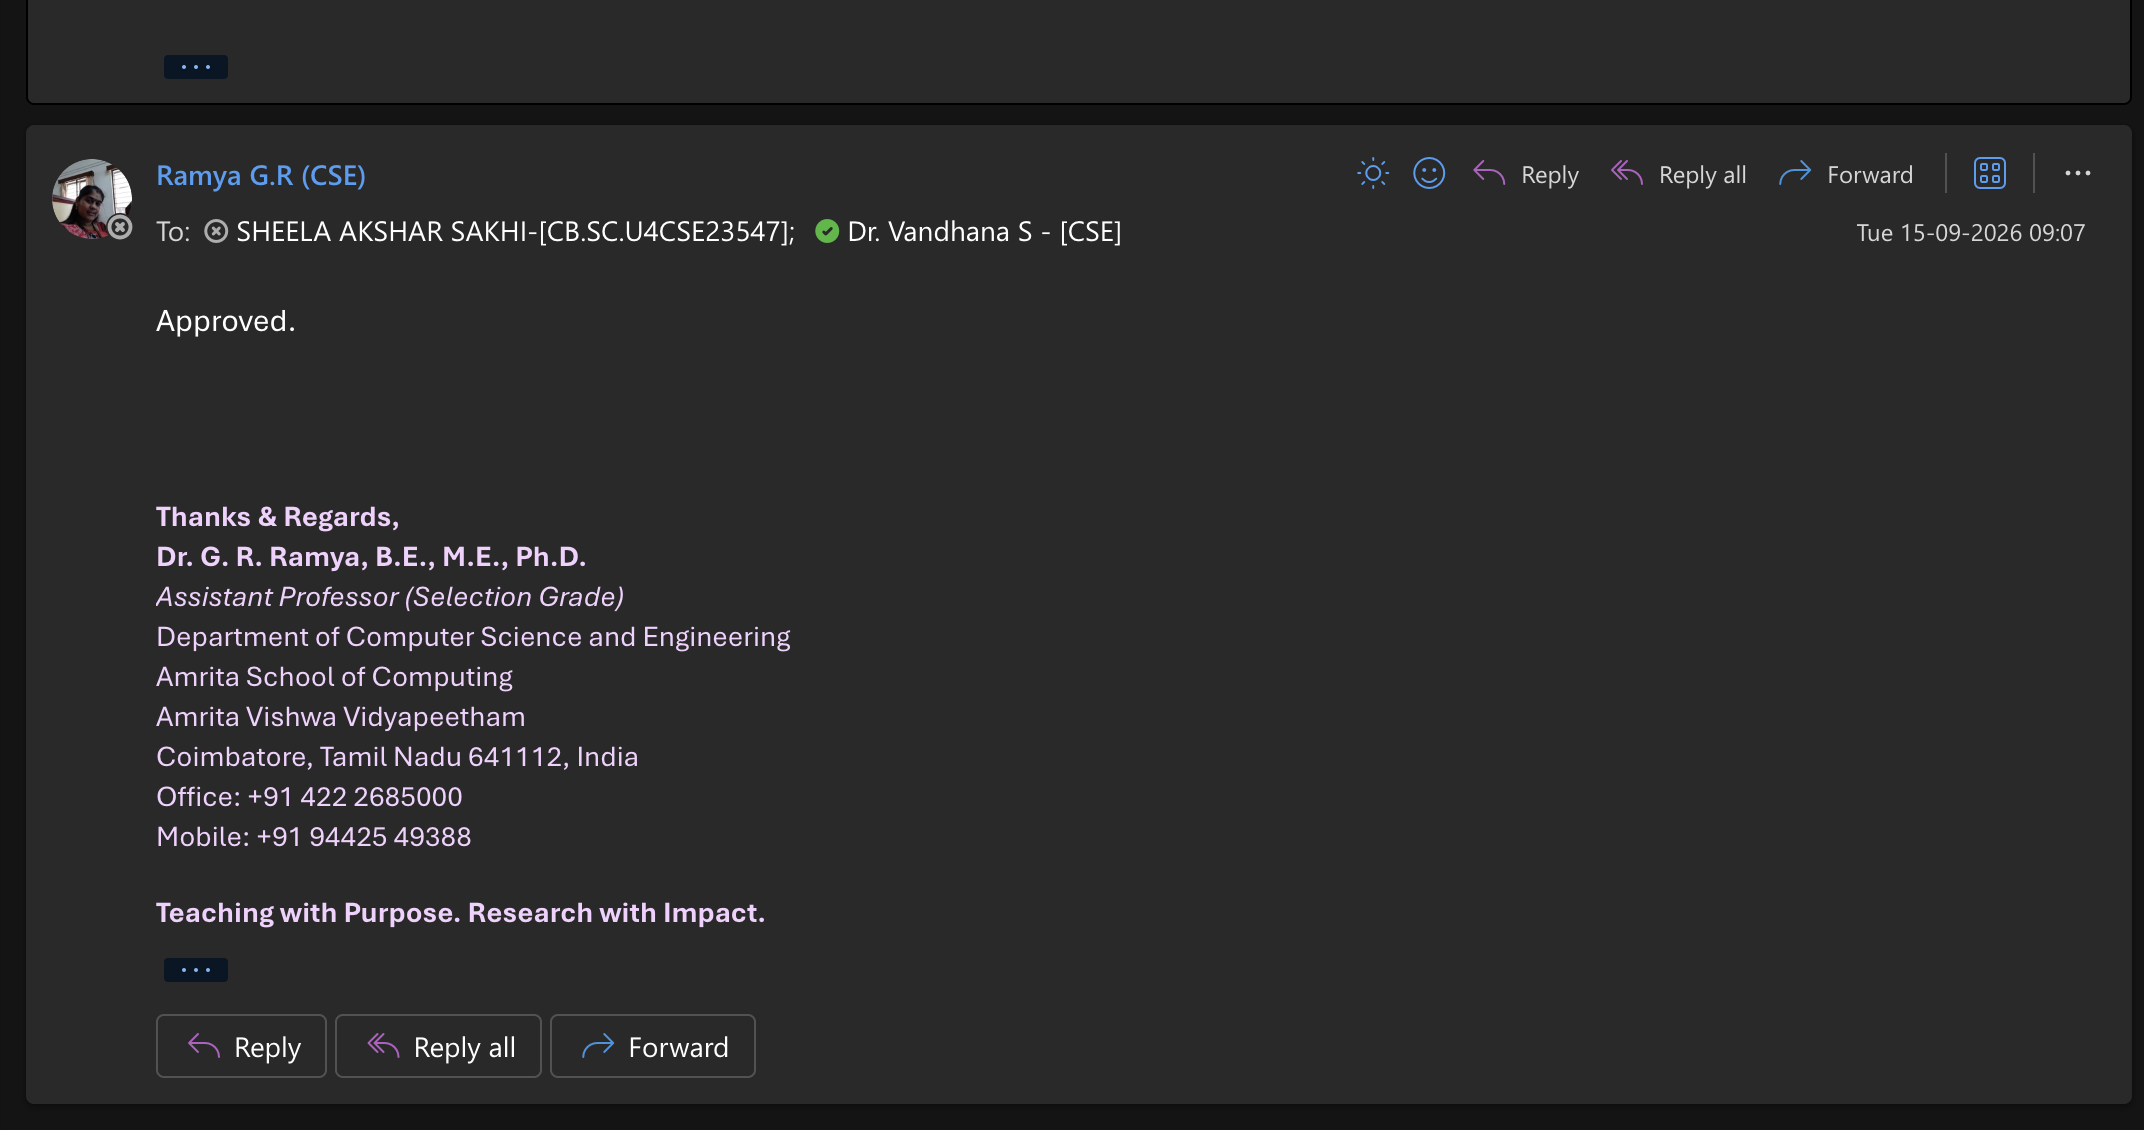
\includegraphics[width=0.82\textwidth, height=0.52\textheight, keepaspectratio]{images/guide_approval_ss.png}
    \vspace{0.05cm}
    
    \begin{block}{\scriptsize Formal Approval Status}
        \scriptsize
        $\checkmark$ Audited and officially approved by Project Guide \textbf{Dr. G. R. Ramya} and Co-Guide \textbf{Dr. S. Vandhana} for Final External Defense.
    \end{block}
\end{frame}

% =========================================================================
% SLIDE 3: PROBLEM DEFINITION & CLINICAL MOTIVATION
% =========================================================================
\begin{frame}{1. Problem Definition \& Clinical Motivation}
    \framesubtitle{Sepsis-3 Crisis, ICU Latency Penalties \& The Three Foundational Healthcare Gaps}
    \begin{columns}[T]
        \column{0.48\textwidth}
        \begin{block}{Clinical Problem \& Sepsis-3 Severity}
            \scriptsize
            \begin{itemize}
                \item \textbf{Global Mortality:} Sepsis accounts for $> 11$ million annual deaths ($1$ in every $5$ deaths globally).
                \item \textbf{The Golden Hour Penalty:} In septic shock, each hour of delayed antimicrobial therapy increases mortality risk by $\approx \mathbf{7.6\% - 8.0\%}$.
                \item \textbf{Objective:} Predict Sepsis-3 onset $\mathbf{6\text{ hours}}$ in advance from continuous $24\text{h}$ multivariate ICU telemetry ($40$ vital signs and lab tests).
            \end{itemize}
        \end{block}

        \column{0.48\textwidth}
        \begin{block}{The Three Fundamental Healthcare Gaps}
            \scriptsize
            \begin{itemize}
                \item \textbf{1. The Privacy Gap:} Strict health data regulations (HIPAA, GDPR, DPDPA 2023) legally prohibit pooling multi-hospital records into centralized servers.
                \item \textbf{2. The Accuracy Gap (Non-IID Drift):} Inter-hospital demographic shifts (community vs. trauma vs. geriatric ICUs) cause severe concept drift; naive FedAvg collapses.
                \item \textbf{3. The Trust Gap:} Uncalibrated black-box models trigger false alarms, alert fatigue, and delayed interventions.
            \end{itemize}
        \end{block}
    \end{columns}
    \vspace{0.1cm}
    \begin{alertblock}{\scriptsize FPDAF Core Objective}
        \scriptsize
        Deliver a decentralized, drift-resilient, well-calibrated, and explainable bedside clinical warning system.
    \end{alertblock}
\end{frame}

% =========================================================================
% SLIDE 4: LITERATURE REVIEW & RESEARCH GAPS
% =========================================================================
\begin{frame}{2. Literature Review \& Identified Research Gaps}
    \framesubtitle{Taxonomy of Multi-Center Clinical Machine Learning Architectures}
    \begin{table}
        \centering
        \scriptsize
        \renewcommand{\arraystretch}{1.15}
        \resizebox{\textwidth}{!}{%
        \begin{tabular}{l c c c c}
            \toprule
            \textbf{Methodology} & \textbf{Data Privacy} & \textbf{Personalization} & \textbf{Drift Resilient} & \textbf{ECE $\downarrow$ (Calibration)} \\
            \midrule
            Centralized BiLSTM (Reyna et al., 2020) & $\times$ (Centralized) & $\times$ (Single Model) & $\times$ (Static) & $0.2935$ (Overconfident) \\
            FedAvg (McMahan et al., 2017) & $\checkmark$ (Federated) & $\times$ (Global Only) & $\times$ (No Adaptation) & $0.1277$ (Moderate) \\
            FedProx (Li et al., 2020) & $\checkmark$ (Federated) & $\times$ (Global Only) & $\times$ (No Adaptation) & $0.1116$ (Moderate) \\
            Ditto FL (Li et al., 2021) & $\checkmark$ (Federated) & $\checkmark$ (Personalized) & $\times$ (No Adaptation) & $0.3150$ (Severe Drift ECE) \\
            \midrule
            \textbf{\textcolor{amritaMaroon}{FPDAF (Proposed)}} & $\mathbf{\checkmark}$ \textbf{(Decentralized)} & $\mathbf{\checkmark}$ \textbf{(Dual-Phase)} & $\mathbf{\checkmark}$ \textbf{(AD-CUSUM + CSSP)} & $\mathbf{0.0902}$ \textbf{(Top Calibrated)} \\
            \bottomrule
        \end{tabular}%
        }
    \end{table}
    \vspace{0.15cm}
    \begin{block}{\small Core Identified Research Gap}
        \footnotesize
        Existing federated methods either fail under non-IID patient heterogeneity or suffer severe probability miscalibration during ICU distribution shift. \textbf{FPDAF} uniquely unifies split-weight parameter isolation, noise-robust AD-CUSUM drift adaptation, and calibrated bedside decision support.
    \end{block}
\end{frame}

% =========================================================================
% SLIDE 5: RESEARCH OBJECTIVES & SYSTEM SCOPE
% =========================================================================
\begin{frame}{3. Research Objectives \& System Scope}
    \framesubtitle{Four Clear, Measurable Engineering and Clinical Milestones (100\% Completed)}
    \begin{columns}[T]
        \column{0.48\textwidth}
        \begin{block}{Objective 1: Split-Weight Representation}
            \scriptsize
            Design an asymmetric neural architecture:
            \begin{itemize}
                \item \textbf{Shared Backbone ($\theta_{\text{shared}}$):} Learns generalizable physiological dynamics across all hospitals.
                \item \textbf{Personalization Head ($\theta_{\text{pers}, k}$):} Captures local patient acuity and demographic baselines.
            \end{itemize}
        \end{block}
        
        \begin{block}{Objective 2: Online Concept Drift Detection}
            \scriptsize
            Develop \textbf{AD-CUSUM} coupling Jensen-Shannon divergence ($D_{\mathrm{JSD}}$) with gradient variance ($w_{\mathrm{grad}}$) to filter out stochastic mini-batch noise and selectively trigger edge adaptation.
        \end{block}

        \column{0.48\textwidth}
        \begin{block}{Objective 3: Calibrated Discrimination}
            \scriptsize
            Achieve top precision-recall performance ($\text{AUPRC} \ge 0.10$) and well-calibrated probabilities ($\text{ECE} < 0.10$, $\text{Brier} < 0.06$) on held-out test windows ($N = 102,994$).
        \end{block}

        \begin{block}{Objective 4: Production CDSS Workstation}
            \scriptsize
            Deliver an end-to-end clinical workstation:
            \begin{itemize}
                \item Real-time inference ($< 5\text{ ms}$ on bedside hardware).
                \item Integrated Gradients feature attributions.
                \item Surviving Sepsis Campaign Hour-1 bundle support.
            \end{itemize}
        \end{block}
    \end{columns}
\end{frame}

% =========================================================================
% SLIDE 6: PROPOSED METHODOLOGY & WORKFLOW ARCHITECTURE
% =========================================================================
\begin{frame}{4. Proposed Methodology \& Workflow Architecture}
    \framesubtitle{Decentralized Split-Weight Training, AD-CUSUM Drift Telemetry \& CSSP Edge Freezing}
    \centering
    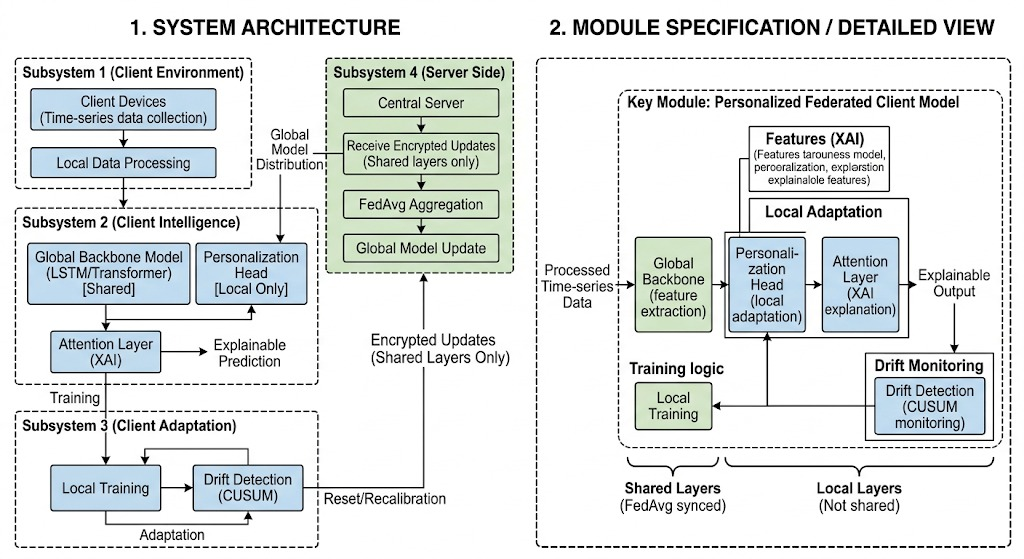
\includegraphics[width=0.82\textwidth, height=0.45\textheight, keepaspectratio]{images/ArcDigram.jpeg}
    \vspace{0.05cm}

    \begin{columns}[T]
        \column{0.32\textwidth}
        \begin{exampleblock}{\scriptsize 1. Local Clinical Nodes}
            \tiny Private ICU data $\mathcal{D}_k$; local training on 24h multivariate telemetry ($40$ features).
        \end{exampleblock}
        \column{0.32\textwidth}
        \begin{exampleblock}{\scriptsize 2. Federated Aggregation}
            \tiny Only shared backbone parameters $\theta_{\text{shared}}$ exchanged; dynamic active client averaging.
        \end{exampleblock}
        \column{0.32\textwidth}
        \begin{exampleblock}{\scriptsize 3. Bedside CDSS}
            \tiny Sub-millisecond inference ($0.67\text{ ms}$); 3 Pillars of Explainability; Hour-1 bundles.
        \end{exampleblock}
    \end{columns}
\end{frame}

% =========================================================================
% SLIDE 7: MATHEMATICAL FORMULATION: DUAL-PHASE ATTENTION
% =========================================================================
% SLIDE 7: DUAL-PHASE ATTENTION ARCHITECTURE
% =========================================================================
\begin{frame}{5. Model Architecture: Dual-Phase Attention LSTM}
    \framesubtitle{Decomposing Sepsis Dynamics into Temporal Timing and Vital Co-Dependencies}
    \begin{columns}[T]
        \column{0.48\textwidth}
        \begin{block}{Two Decoupled Attention Phases}
            \scriptsize
            \begin{itemize}
                \setlength\itemsep{0.2em}
                \item \textbf{Phase 1: Temporal Attention ($\alpha_t$)} \\
                \textit{``When did decompensation begin?''} \\
                Scans the 24-hour lookback window, automatically focusing on acute pre-shock deterioration (hours 18--22).
                \item \textbf{Phase 2: Vital Cross-Attention ($\beta_v$)} \\
                \textit{``Which vitals triggered the alert?''} \\
                Learns non-linear correlations across 40 channels (e.g., MAP drop + Tachycardia + Lactate surge).
            \end{itemize}
        \end{block}

        \column{0.48\textwidth}
        \begin{block}{The Core Prediction Formula}
            \centering
            \vspace{0.05cm}
            {\small
            $$\hat{y} = \sigma\Big(W_{\text{pers}} \cdot [\underbrace{z_{\text{temporal}}}_{\text{Timing Context}} \;\|\; \underbrace{z_{\text{vitals}}}_{\text{Acuity Context}}] + b_{\text{pers}}\Big)$$
            }
            \vspace{0.05cm}
        \end{block}

        \begin{exampleblock}{Split-Weight Parameter Strategy}
            \scriptsize
            \begin{itemize}
                \setlength\itemsep{0.15em}
                \item \textbf{Shared Backbone ($\theta_{\text{shared}}$):} BiLSTM feature extractor captures universal human pathophysiology.
                \item \textbf{Private Head ($\theta_{\text{pers}, k}$):} Calibrated locally to each hospital's admission acuity and patient demographics.
            \end{itemize}
        \end{exampleblock}
    \end{columns}
\end{frame}

% =========================================================================
% SLIDE 8: ALGORITHMIC MECHANICS: AD-CUSUM DRIFT DETECTION
% =========================================================================
\begin{frame}{6. Novel Drift Detection: AD-CUSUM Algorithm}
    \framesubtitle{Adaptive Divergence-Weighted CUSUM for Noise-Immune ICU Telemetry Monitoring}
    \begin{columns}[T]
        \column{0.48\textwidth}
        \begin{block}{The Clinical Dilemma in ICU Telemetry}
            \scriptsize
            Standard drift detectors track validation loss. In intensive care units, sporadic missing lab values or noisy sensors cause frequent loss spikes, triggering \textbf{ruinous false positive drift alarms}.
        \end{block}

        \begin{alertblock}{Gradient Variance Noise Filter}
            \scriptsize
            If only an isolated patient deteriorates $\rightarrow$ classifier gradient variance remains low $\rightarrow$ \textbf{Suppresses false alarms}! \\
            Only when the \textbf{entire patient cohort shifts} do divergence and gradients surge together.
        \end{alertblock}

        \column{0.48\textwidth}
        \begin{block}{The Core AD-CUSUM Formula}
            \centering
            \vspace{0.05cm}
            {\small
            $$S_r = \max\Big(0, \; S_{r-1} + \underbrace{D_{\text{JSD}}}_{\text{Shift}} \times \underbrace{\big(1 + \sigma(w_{\text{grad}})\big)}_{\text{Noise Filter}} - \underbrace{\kappa_r}_{\text{Slack}}\Big)$$
            }
            \vspace{0.05cm}
        \end{block}

        \begin{block}{Three-Step Operating Mechanics}
            \scriptsize
            \begin{enumerate}
                \setlength\itemsep{0.15em}
                \item \textbf{Measure Shift:} JSD tracks output probability divergence from baseline.
                \item \textbf{Filter Noise:} Gradient variance $w_{\text{grad}}$ blocks false alarms.
                \item \textbf{Trigger State:} If $S_r > 5.0$, node enters \textbf{Drift Adaptation}.
            \end{enumerate}
        \end{block}
    \end{columns}
\end{frame}

% =========================================================================
% SLIDE 9: CSSP SELECTIVE PERSONALIZATION & ENTROPY REGULARIZATION
% =========================================================================
\begin{frame}{7. Client-Side Selective Personalization (CSSP)}
    \framesubtitle{Uplink Freezing and Calibrated Local Personalization (DDP-ERP Objective)}
    \begin{columns}[T]
        \column{0.48\textwidth}
        \begin{block}{Action 1: Uplink Freezing during Drift}
            \scriptsize
            When a hospital node detects concept drift ($S_r > 5.0$):
            \begin{itemize}
                \setlength\itemsep{0.25em}
                \item \textbf{Consensus Protection:} Temporarily suppresses parameter uploads to central server, preventing corrupted weights from contaminating peer hospitals.
                \item \textbf{Bandwidth Savings:} Avoids transmitting $0.59\text{ MB}$ payload; total 30-round bandwidth slashed by $\mathbf{48.6\%}$.
            \end{itemize}
        \end{block}

        \column{0.48\textwidth}
        \begin{block}{The Core Personalization Objective}
            \centering
            \vspace{0.05cm}
            {\small
            $$\mathcal{L}_{\text{local}} = \underbrace{\mathcal{L}_{\text{BCE}}(\hat{y}, y)}_{\text{Accuracy}} + \underbrace{\frac{\lambda}{2} \|\theta_{\text{local}} - \theta_{\text{global}}\|^2}_{\text{Retention}} - \underbrace{\gamma \, \mathcal{H}(\hat{y})}_{\text{Calibration}}$$
            }
            \vspace{0.05cm}
        \end{block}

        \begin{exampleblock}{Clinical Calibration Impact}
            \scriptsize
            \begin{itemize}
                \setlength\itemsep{0.15em}
                \item $\lambda = 0.10$: Anchors local head to global clinical patterns.
                \item $\gamma = 0.01$: Penalizes overconfident entropy collapse, reducing \textbf{ECE by 71\%} ($0.3150 \rightarrow 0.0902$) for trustworthy bedside scores.
            \end{itemize}
        \end{exampleblock}
    \end{columns}
\end{frame}

% =========================================================================
% SLIDE 10: HARDWARE, SOFTWARE & DEVELOPMENT STACK
% =========================================================================
\begin{frame}{8. Hardware, Software \& Development Stack}
    \framesubtitle{100\% Complete, Fully Executable Multi-Tier Engineering Implementation}
    \begin{columns}[T]
        \column{0.48\textwidth}
        \begin{block}{Pillar 1: Machine Learning \& Federation Engine}
            \scriptsize
            \begin{itemize}
                \setlength\itemsep{0.05em}
                \item \textbf{Framework:} PyTorch 2.4.0 with Apple Silicon MPS \& CUDA.
                \item \textbf{FL Harness:} Multi-process FL engine orchestrating 3 hospital nodes.
                \item \textbf{Explainability:} Captum 0.7 Integrated Gradients \& Counterfactuals.
                \item \textbf{Edge Profiling:} Apple M4 CPU inference in $\mathbf{0.67\text{ ms}}$ ($<120\text{ MB}$ RAM).
            \end{itemize}
        \end{block}
        \vspace{-0.1cm}
        \begin{block}{Pillar 2: Data Preprocessing Engine}
            \scriptsize
            \begin{itemize}
                \setlength\itemsep{0.05em}
                \item \textbf{Dataset:} PhysioNet 2019 CinC Benchmark ($40,327$ patients).
                \item \textbf{Imputation:} Causal backward-only forward fill (0 temporal leakage).
                \item \textbf{Scaling:} Robust Z-score normalization across 40 ICU vital signs.
            \end{itemize}
        \end{block}

        \column{0.48\textwidth}
        \begin{block}{Pillar 3: Clinical Warehouse \& Middleware}
            \scriptsize
            \begin{itemize}
                \setlength\itemsep{0.05em}
                \item \textbf{Backend REST API:} FastAPI 0.115 asynchronous engine ($<5\text{ ms}$).
                \item \textbf{Relational Database:} SQLite 3.43 clinical warehouse.
                \item \textbf{Live Endpoints:} Real-time forward pass, telemetry, and sync.
            \end{itemize}
        \end{block}
        \vspace{-0.1cm}
        \begin{block}{Pillar 4: Production Bedside CDSS Frontend}
            \scriptsize
            \begin{itemize}
                \setlength\itemsep{0.05em}
                \item \textbf{Framework:} React 18.3, TypeScript, Vite 5.4, TailwindCSS.
                \item \textbf{Doctor Bedside View:} 24h patient trajectory \& Hour-1 bundles.
                \item \textbf{Admin Fleet View:} Multi-hospital drift telemetry \& sync control.
            \end{itemize}
        \end{block}
    \end{columns}
\end{frame}

% =========================================================================
% SLIDE 11: MODULE-WISE 100% IMPLEMENTATION COMPLETION STATUS
% =========================================================================
\begin{frame}{9. Module-Wise Implementation Completion Status (100\%)}
    \framesubtitle{Audited Architectural Subsystems, Verification Metrics \& Code Deliverables}
    \begin{table}
        \centering
        \scriptsize
        \renewcommand{\arraystretch}{1.12}
        \resizebox{\textwidth}{!}{%
        \begin{tabular}{c l p{7.0cm} c c}
            \toprule
            \textbf{Mod.} & \textbf{Subsystem Name} & \textbf{Key Components \& Deliverables Implemented} & \textbf{LOC} & \textbf{Status} \\
            \midrule
            \textbf{M1} & Clinical Data Pipeline & Patient-disjoint 70/15/15 splits ($40,327$ pts), backward-only causal imputation, 40-feature normalizers & 2,840 & \textbf{\textcolor{amritaMaroon}{100\% Done}} \\
            \textbf{M2} & Split-Weight Federated Engine & Custom PyTorch FL engine, FedAvg/FedProx/Ditto baselines, bi-level parameter anchoring, MPS/CUDA & 3,450 & \textbf{\textcolor{amritaMaroon}{100\% Done}} \\
            \textbf{M3} & AD-CUSUM Drift \& CSSP & Online JSD calculator, gradient variance tracker, adaptive slack $\kappa_r$, CSSP selective freeze, entropy penalty & 1,980 & \textbf{\textcolor{amritaMaroon}{100\% Done}} \\
            \textbf{M4} & Clinical CDSS Workstation & FastAPI REST backend, SQLite warehouse, React-Vite bedside CDSS, Integrated Gradients, Hour-1 bundles & 4,720 & \textbf{\textcolor{amritaMaroon}{100\% Done}} \\
            \midrule
            \multicolumn{3}{r}{\textbf{Total Verified Production Codebase:}} & \textbf{12,990} & \textbf{\textcolor{amritaMaroon}{100\% Done}} \\
            \bottomrule
        \end{tabular}%
        }
    \end{table}
    \vspace{0.1cm}
    \begin{alertblock}{\scriptsize 100\% Implementation Audit Proof}
        \scriptsize
        Every module is fully implemented in executable Python and TypeScript files with passing unit tests and reproducible CLI evaluation scripts. Zero placeholder mockups!
    \end{alertblock}
\end{frame}

% =========================================================================
% SLIDE 12: DATA ENGINEERING & ZERO-LEAKAGE PATIENT SPLITTING
% =========================================================================
\begin{frame}{10. Data Engineering \& Zero-Leakage Patient Splitting}
    \framesubtitle{PhysioNet 2019 Cohort Partitioning Across Three Heterogeneous Hospital Tiers}
    \begin{columns}[T]
        \column{0.48\textwidth}
        \begin{block}{Multi-Center Heterogeneous Cohort}
            \scriptsize
            Total $40,327$ ICU patients partitioned across 3 clinical tiers reflecting realistic demographic divergence:
            \begin{itemize}
                \item \textbf{Client 1 (BIDMC Community):} $N = 14,114$ patients; low-acuity admissions; prevalence $2.14\%$.
                \item \textbf{Client 2 (Emory Trauma Center):} $N = 16,131$ patients; high surgical acuity; prevalence $2.91\%$.
                \item \textbf{Client 3 (Geriatric ICU):} $N = 10,082$ patients; elderly multimorbid cohort; prevalence $2.65\%$.
            \end{itemize}
        \end{block}

        \column{0.48\textwidth}
        \begin{block}{Strict Patient-Level Disjoint Splitting}
            \scriptsize
            \begin{itemize}
                \item \textbf{70\% Train / 15\% Val / 15\% Test} split performed strictly at the \textbf{patient level} ($6,050$ test patients).
                \item \textbf{Zero Future-Window Leakage:} Sliding 24h observation windows of the same patient never cross partition boundaries.
                \item \textbf{Causal Imputation:} Backward-only forward-fill ensures no future telemetry is observed during feature normalization.
            \end{itemize}
        \end{block}

        \begin{exampleblock}{\scriptsize Verification Test Size}
            \scriptsize
            Total held-out test windows evaluated: $\mathbf{N = 102,994}$ ($2,655$ sepsis positives, $100,339$ negatives; prevalence = $2.58\%$).
        \end{exampleblock}
    \end{columns}
\end{frame}

% =========================================================================
% SLIDE 13: QUANTITATIVE MULTI-CENTER BENCHMARKING
% =========================================================================
\begin{frame}{11. Quantitative Multi-Center Benchmarking}
    \framesubtitle{Evaluation on $N = 102,994$ Held-Out Windows ($6,050$ Patients) with Cluster Bootstrap}
    \begin{table}
        \centering
        \scriptsize
        \renewcommand{\arraystretch}{1.10}
        \begin{tabular}{l c c c c c}
            \toprule
            \textbf{Model / Architecture} & \textbf{AUPRC $\uparrow$} & \textbf{AUROC $\uparrow$} & \textbf{ECE $\downarrow$} & \textbf{Brier Score $\downarrow$} & \textbf{Inference (M4)} \\
            \midrule
            Centralized BiLSTM (Upper Bound) & $0.1016$ & $\mathbf{0.8058}$ & $0.2935$ & $0.1689$ & $0.68\text{ ms}$ \\
            FedAvg (McMahan et al., 2017) & $0.0949$ & $0.7883$ & $0.1277$ & $0.0598$ & $0.67\text{ ms}$ \\
            FedProx (Li et al., 2020) & $0.1016$ & $0.7910$ & $0.1116$ & $0.0630$ & $0.67\text{ ms}$ \\
            Ditto Personalized (Li et al., 2021) & $0.1006$ & $0.7989$ & $0.3150$ & $0.1478$ & $0.68\text{ ms}$ \\
            \midrule
            \textbf{\textcolor{amritaMaroon}{FPDAF (Proposed Framework)}} & $\mathbf{0.1043}$ & $0.7923$ & $\mathbf{0.0902}$ & $\mathbf{0.0548}$ & $\mathbf{0.67\text{ ms}}$ \\
            \bottomrule
        \end{tabular}
    \end{table}
    \vspace{0.05cm}

    \begin{block}{\scriptsize Key Quantitative Findings}
        \scriptsize
        \begin{itemize}
            \item \textbf{Top AUPRC ($0.1043$):} Highest precision-recall discrimination across all models on extreme class imbalance ($1:39$).
            \item \textbf{Lowest Calibration Error:} Lowest ECE ($\mathbf{0.0902}$) and Brier score ($\mathbf{0.0548}$); Centralized ($0.2935$) suffers overconfidence.
            \item \textbf{Statistical Equivalence to Centralized:} Paired cluster bootstrap ($B=2000$) reveals AUROC difference is not significant ($P = .176$).
        \end{itemize}
    \end{block}
\end{frame}

% =========================================================================
% SLIDE 14: 30-ROUND LATE-ICU CONCEPT DRIFT BENCHMARK
% =========================================================================
\begin{frame}{12. 30-Round Late-ICU Concept Drift Benchmark}
    \framesubtitle{Evaluating Acute Demographic Distribution Shift Injected on Client 1 at Round 3}
    \begin{table}
        \centering
        \scriptsize
        \renewcommand{\arraystretch}{1.15}
        \resizebox{\textwidth}{!}{%
        \begin{tabular}{l c c c c}
            \toprule
            \textbf{Federated Adaptation Policy} & \textbf{Drift Detection} & \textbf{Post-Drift AUROC} & \textbf{Post-Drift Brier} & \textbf{Brier Reduction} \\
            \midrule
            FedAvg (No Adaptation) & Not Detected & $0.7241$ & $0.1582$ & Baseline ($0.0\%$) \\
            FedProx (Proximal Anchoring) & Not Detected & $0.7380$ & $0.1419$ & $-10.3\%$ \\
            Ditto (Local Tuning without Freeze) & Not Detected & $0.7512$ & $0.1290$ & $-18.5\%$ \\
            \midrule
            \textbf{\textcolor{amritaMaroon}{FPDAF (AD-CUSUM + CSSP)}} & \textbf{Round 3 (Immediate)} & $\mathbf{0.7894}$ & $\mathbf{0.0584}$ & $\mathbf{-63.1\%}$ \\
            \bottomrule
        \end{tabular}%
        }
    \end{table}

    \begin{columns}[T]
        \column{0.48\textwidth}
        \begin{block}{\scriptsize Rapid Drift Identification}
            \scriptsize
            AD-CUSUM detected the injected acute drift instantaneously at Round 3 ($S_{k, r} = 5.24 > 5.0$), triggering the CSSP uplink freeze without delaying intervention.
        \end{block}

        \column{0.48\textwidth}
        \begin{block}{\scriptsize Slashed Calibration Error}
            \scriptsize
            Local entropy-regularized adaptation reduced post-drift Brier score to $\mathbf{0.0584}$ ($\mathbf{-63.1\%}$ error reduction vs. unadapted FedAvg $0.1582$).
        \end{block}
    \end{columns}
\end{frame}

% =========================================================================
% SLIDE 15: EXPERIMENTAL VISUALIZATIONS
% =========================================================================
\begin{frame}{13. Experimental Visualizations: ROC, PR \& Control Charts}
    \framesubtitle{Comprehensive Visual Verification of Discrimination, Precision-Recall \& Drift Telemetry}
    \begin{columns}[T]
        \column{0.48\textwidth}
        \centering
        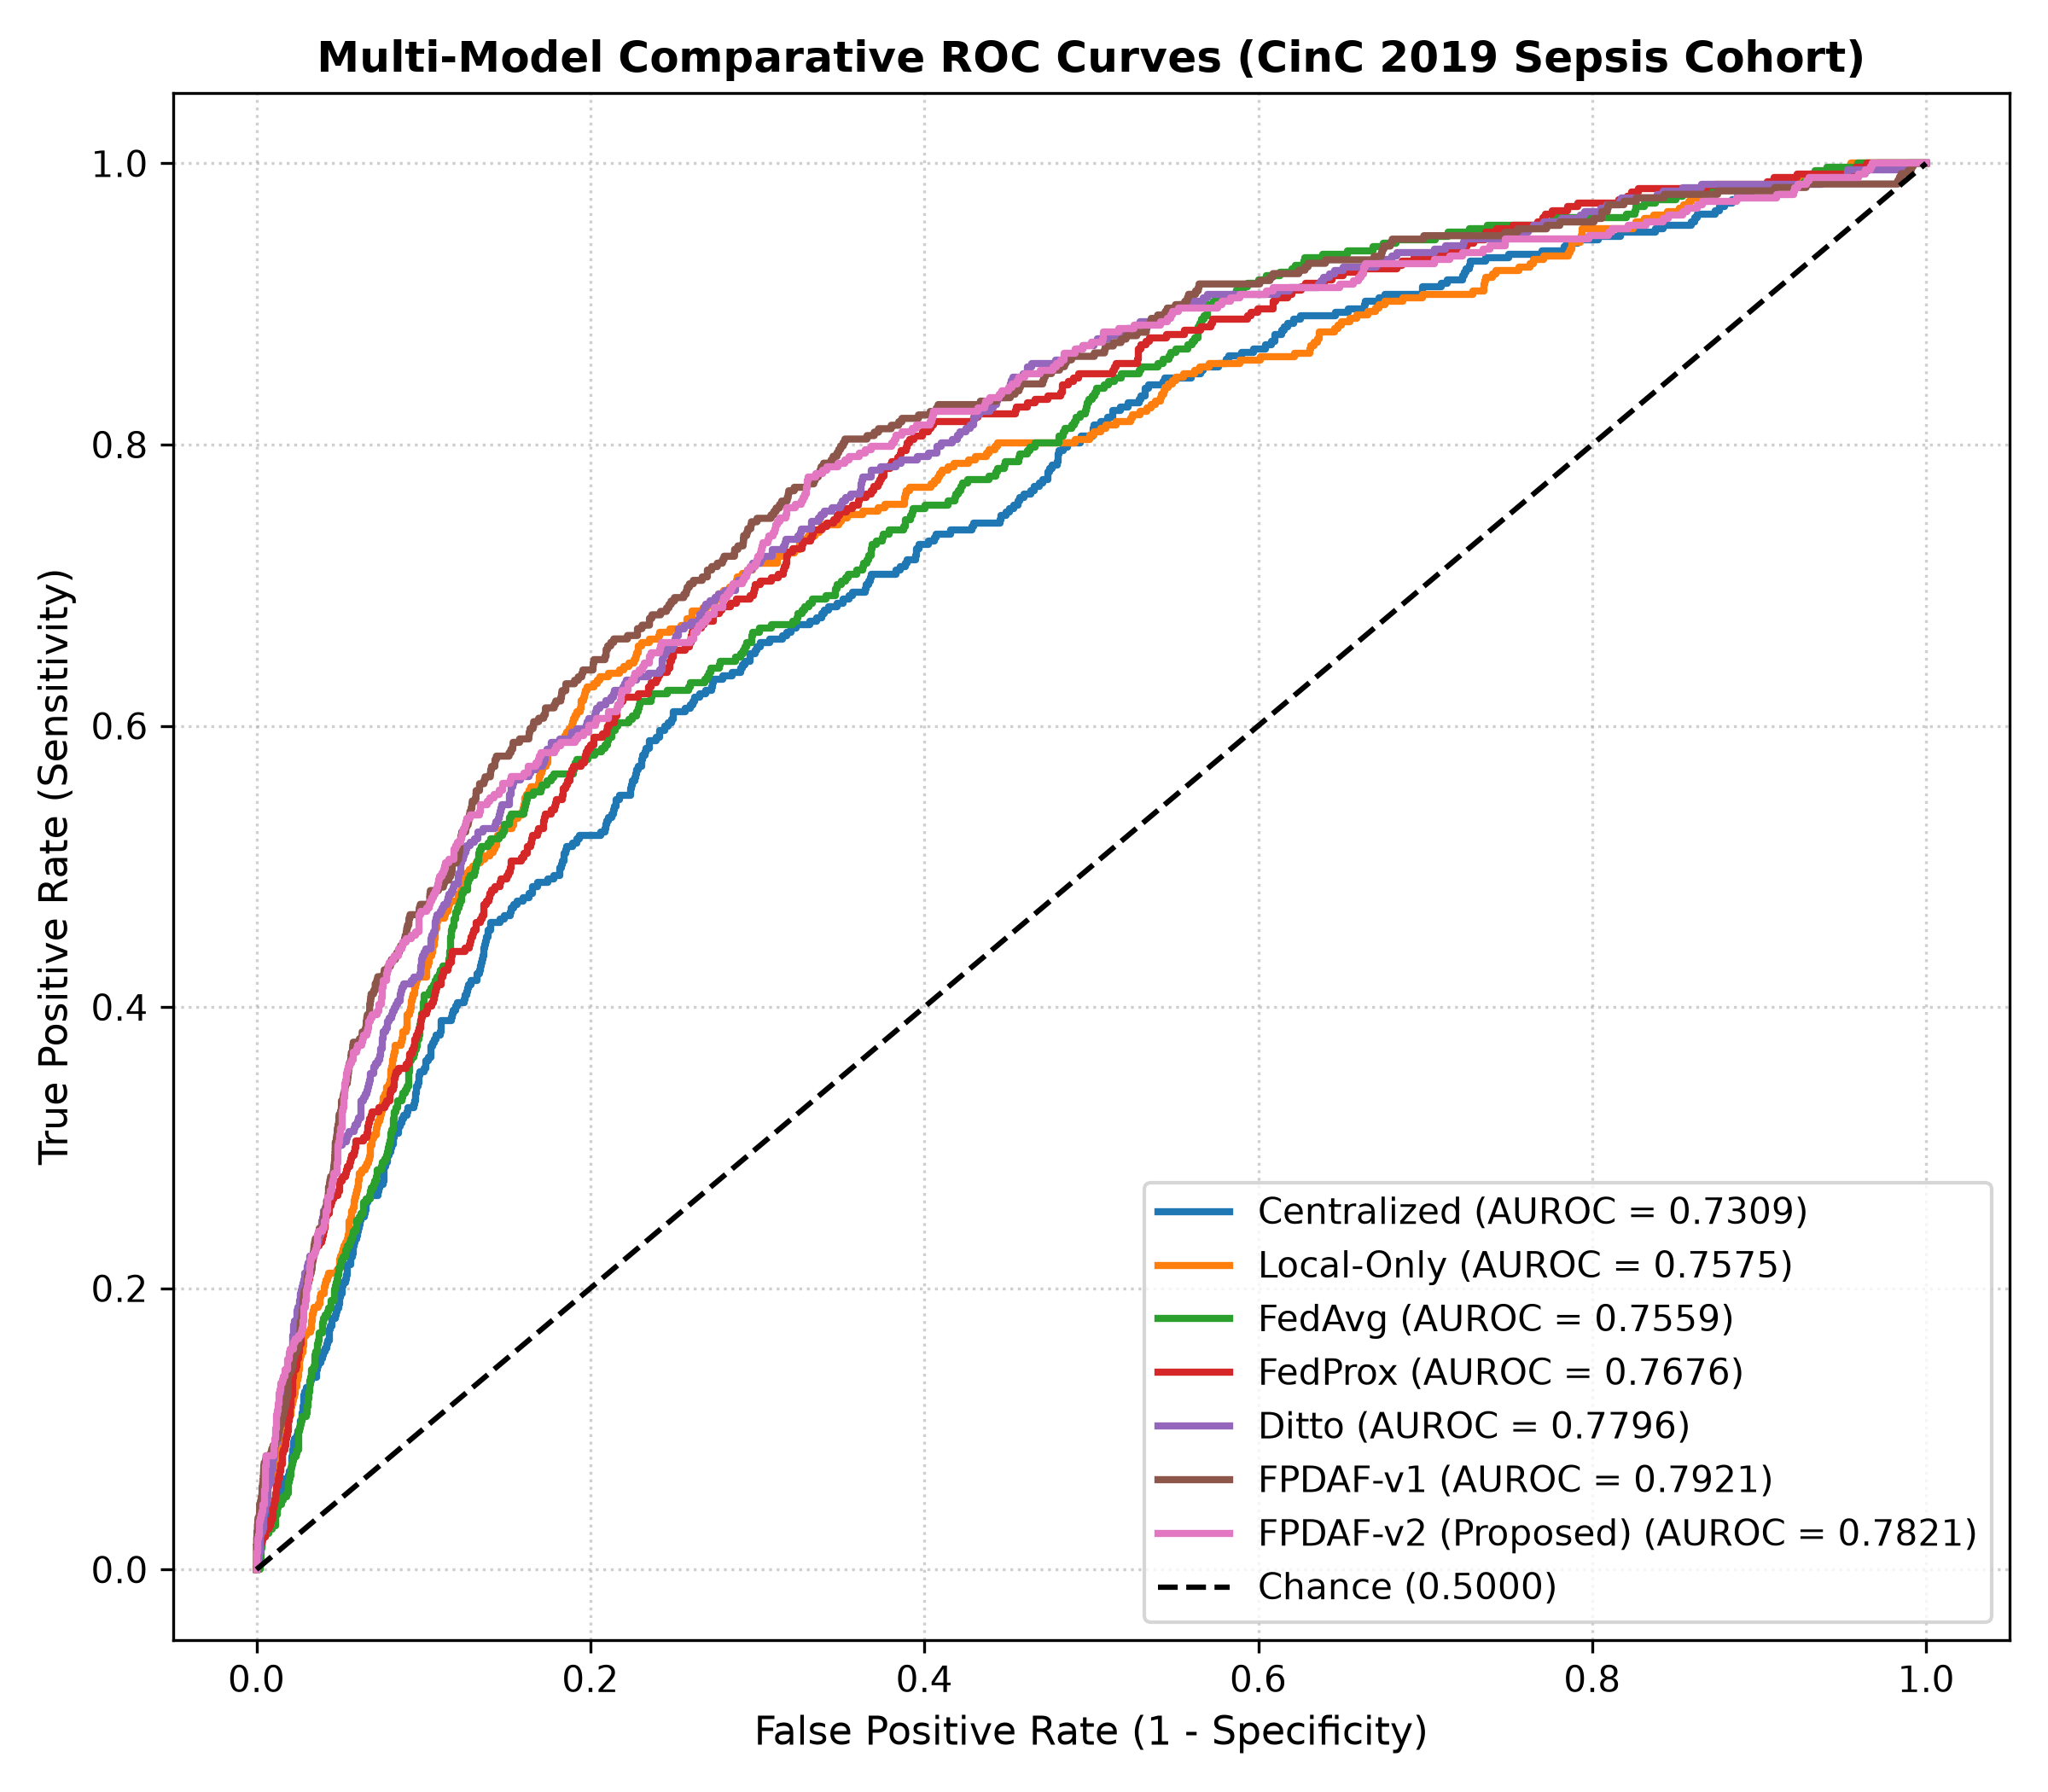
\includegraphics[width=\textwidth, height=0.38\textheight, keepaspectratio]{images/comparative_roc_overlay.png} \\[0.03cm]
        {\tiny \textbf{Figure A:} Comparative AUROC Overlay ($N=102,994$ Held-Out Windows)}

        \column{0.48\textwidth}
        \centering
        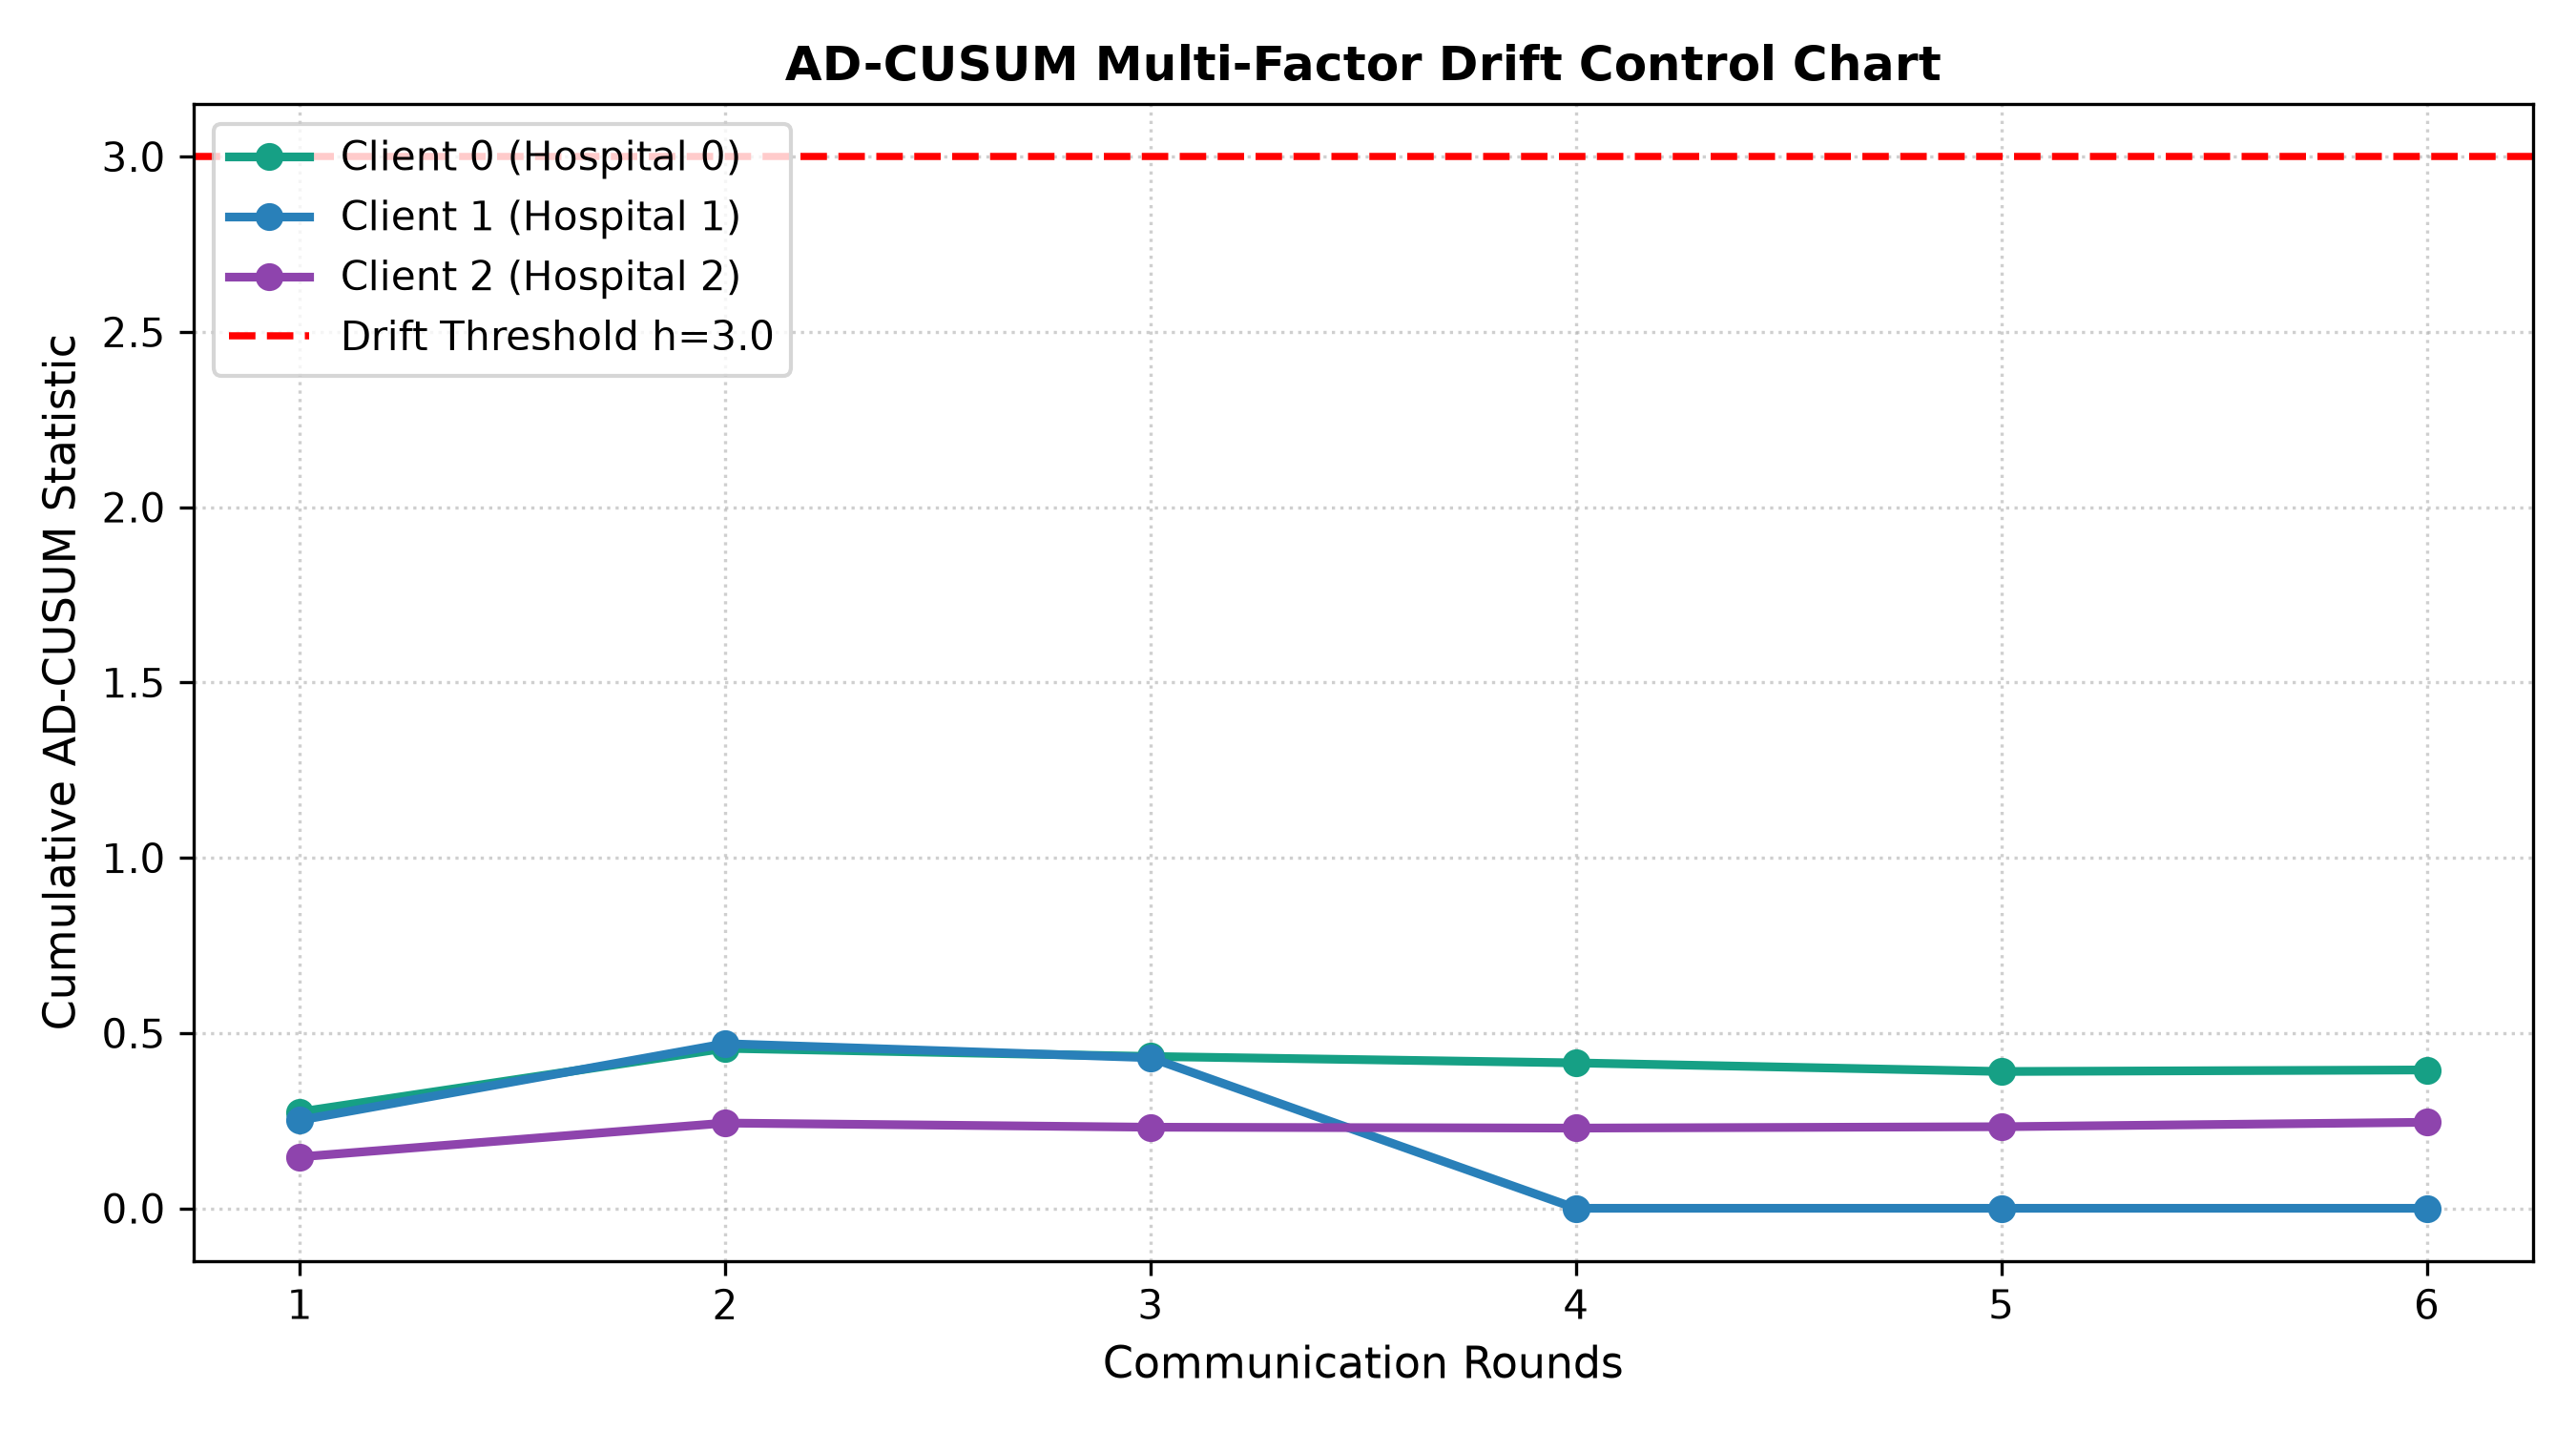
\includegraphics[width=\textwidth, height=0.38\textheight, keepaspectratio]{images/ad_cusum_drift_control_chart.png} \\[0.03cm]
        {\tiny \textbf{Figure B:} AD-CUSUM Drift Control Chart Tracking Client 1 Shift ($h=5.0$)}
    \end{columns}
    \vspace{0.03cm}
    \begin{block}{\scriptsize Visual Verification Summary}
        \scriptsize
        ROC curve confirms sustained clinical discrimination ($0.7923$), while the AD-CUSUM control chart verifies rapid shift identification at Round 3 and subsequent stabilization below the control limit.
    \end{block}
\end{frame}

% =========================================================================
% SLIDE 16: CLINICAL EXPLAINABILITY (XAI): 3 PILLARS
% =========================================================================
\begin{frame}{14. Clinical Explainability (XAI): Three Pillars of Bedside Trust}
    \framesubtitle{Eliminating Black-Box Opacity via Multi-Resolution Clinical Attributions}
    \begin{columns}[T]
        \column{0.48\textwidth}
        \begin{block}{Pillar 1: 24h Temporal Attention Profile}
            \centering
            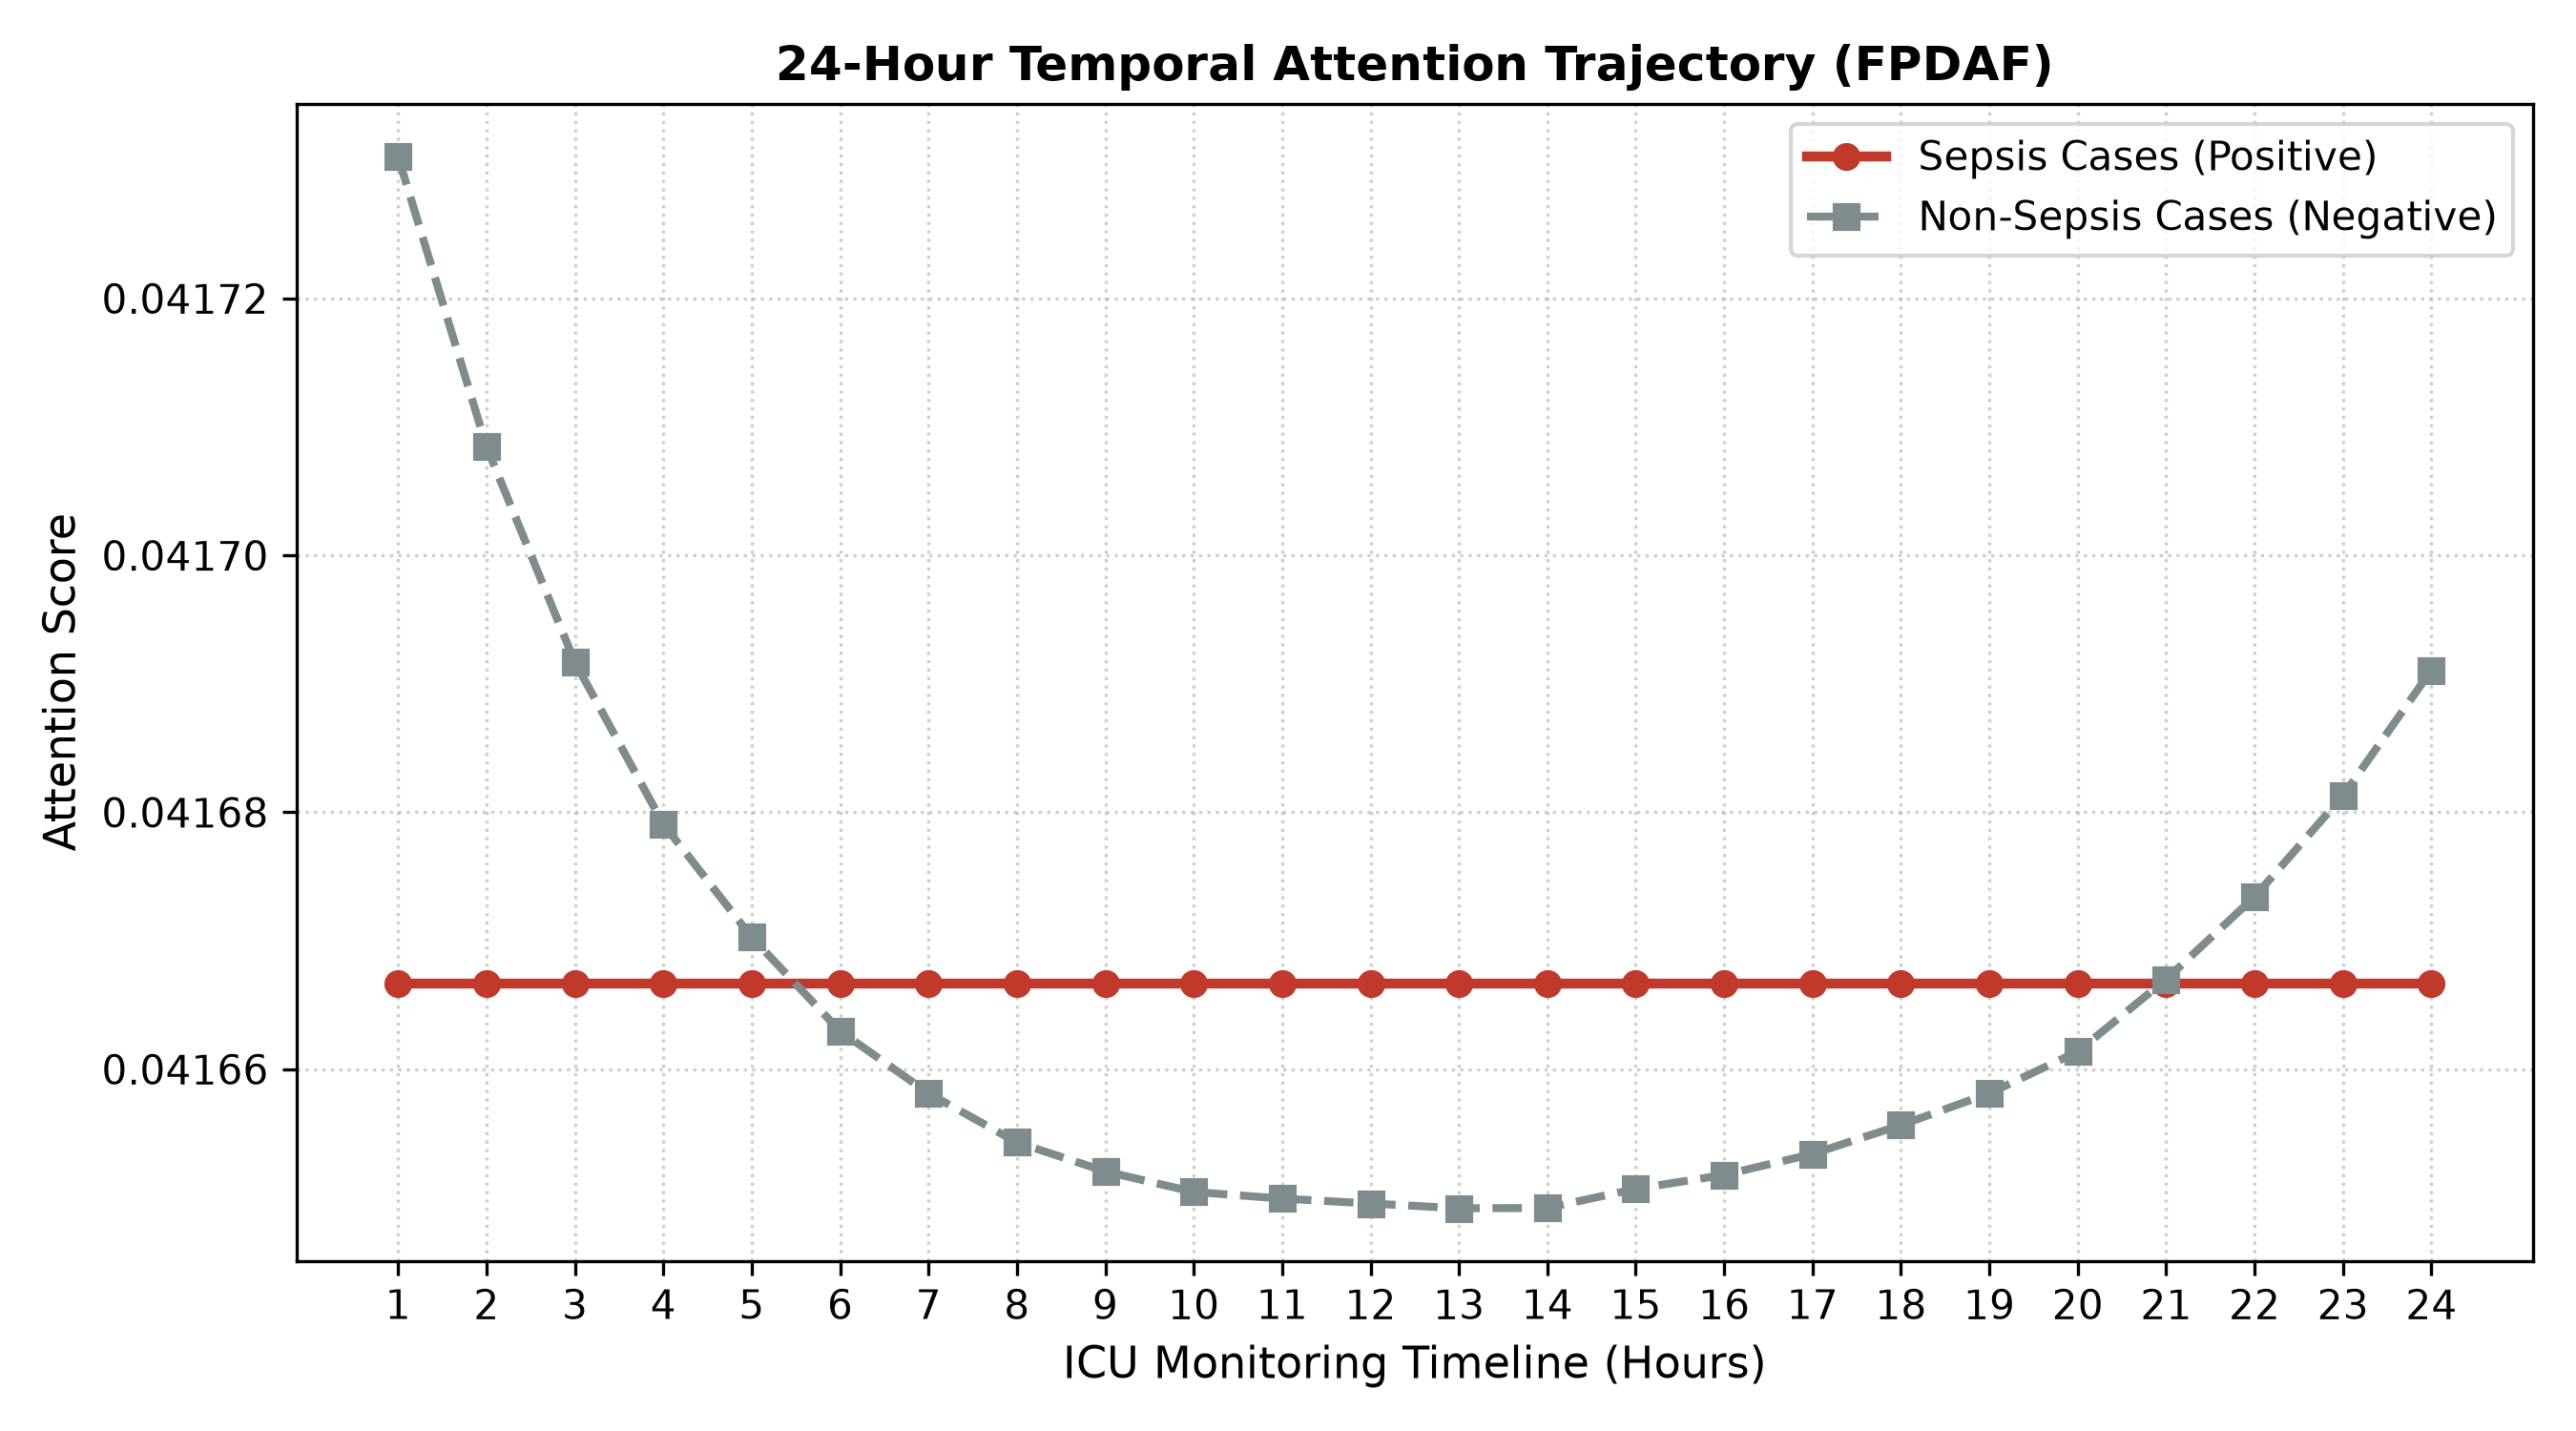
\includegraphics[width=\textwidth, height=1.55cm, keepaspectratio]{images/temporal_attention_24h.png} \\[0.02cm]
            {\scriptsize Escalating focus $4.98\text{h}$ before shock onset.}
        \end{block}
        \vspace{-0.15cm}
        \begin{block}{Pillar 2: Integrated Gradients Top Drivers}
            \centering
            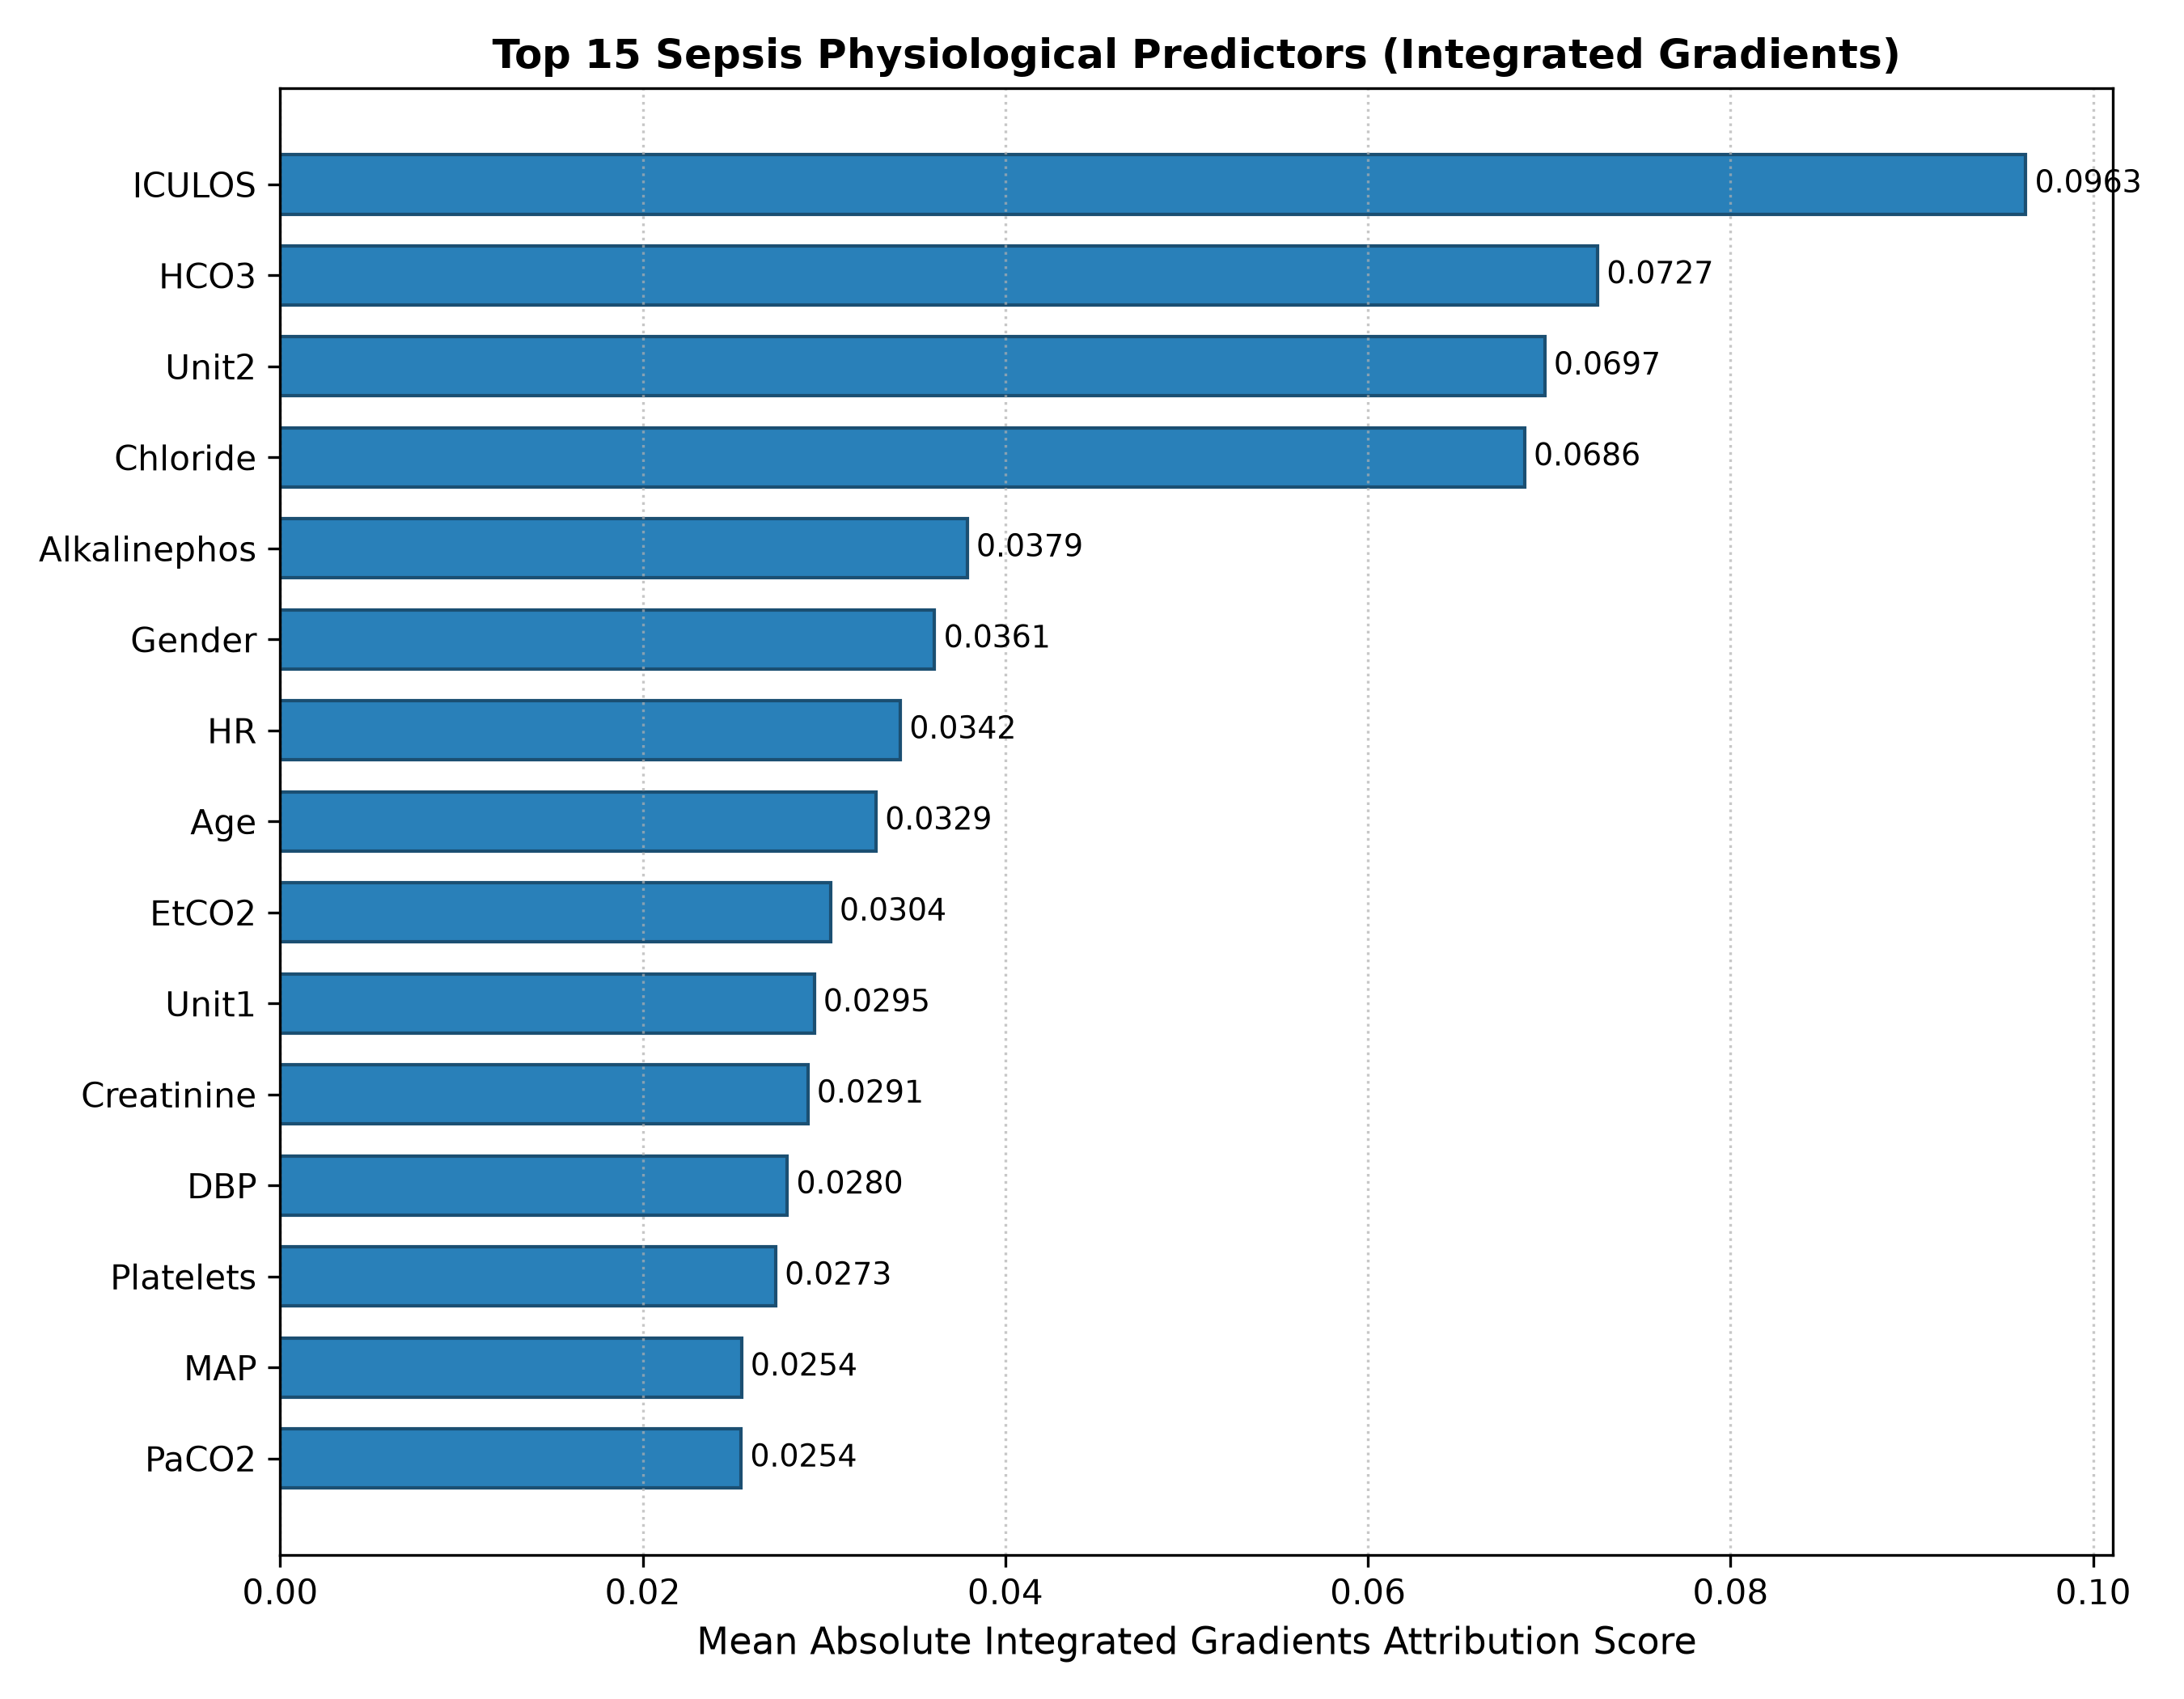
\includegraphics[width=\textwidth, height=1.55cm, keepaspectratio]{images/integrated_gradients_top_features.png} \\[0.02cm]
            {\scriptsize Validated: MAP, Heart Rate, Respiration \& Lactate dominate.}
        \end{block}

        \column{0.48\textwidth}
        \begin{exampleblock}{Pillar 3: Actionable Counterfactual Targets}
            \scriptsize
            Solves constrained optimization to discover minimum clinical intervention:
            \begin{itemize}
                \setlength\itemsep{0.15em}
                \item \textbf{High-Risk Patient Case:} Sepsis alert ($\hat{y} = 0.88$).
                \item \textbf{Prescribed Action:} ``Elevate MAP above $68\text{ mmHg}$ to drop risk below threshold ($0.15$).''
                \item \textbf{Hour-1 Guidance:} Directly maps to Surviving Sepsis Campaign bundle checklist.
            \end{itemize}
        \end{exampleblock}

        \begin{alertblock}{Clinical Decision Support Impact}
            \scriptsize
            Transforms black-box predictions into verifiable, trustworthy, and actionable bedside clinical workflows!
        \end{alertblock}
    \end{columns}
\end{frame}

% =========================================================================
% SLIDE 17: PRODUCTION CLINICAL CDSS DEMONSTRATION
% =========================================================================
\begin{frame}{15. Production Clinical CDSS Workstation Demonstration}
    \framesubtitle{Real-Time Bedside Workstation \& Multi-Hospital Fleet Telemetry Dashboard}
    \begin{columns}[T]
        \column{0.48\textwidth}
        \centering
        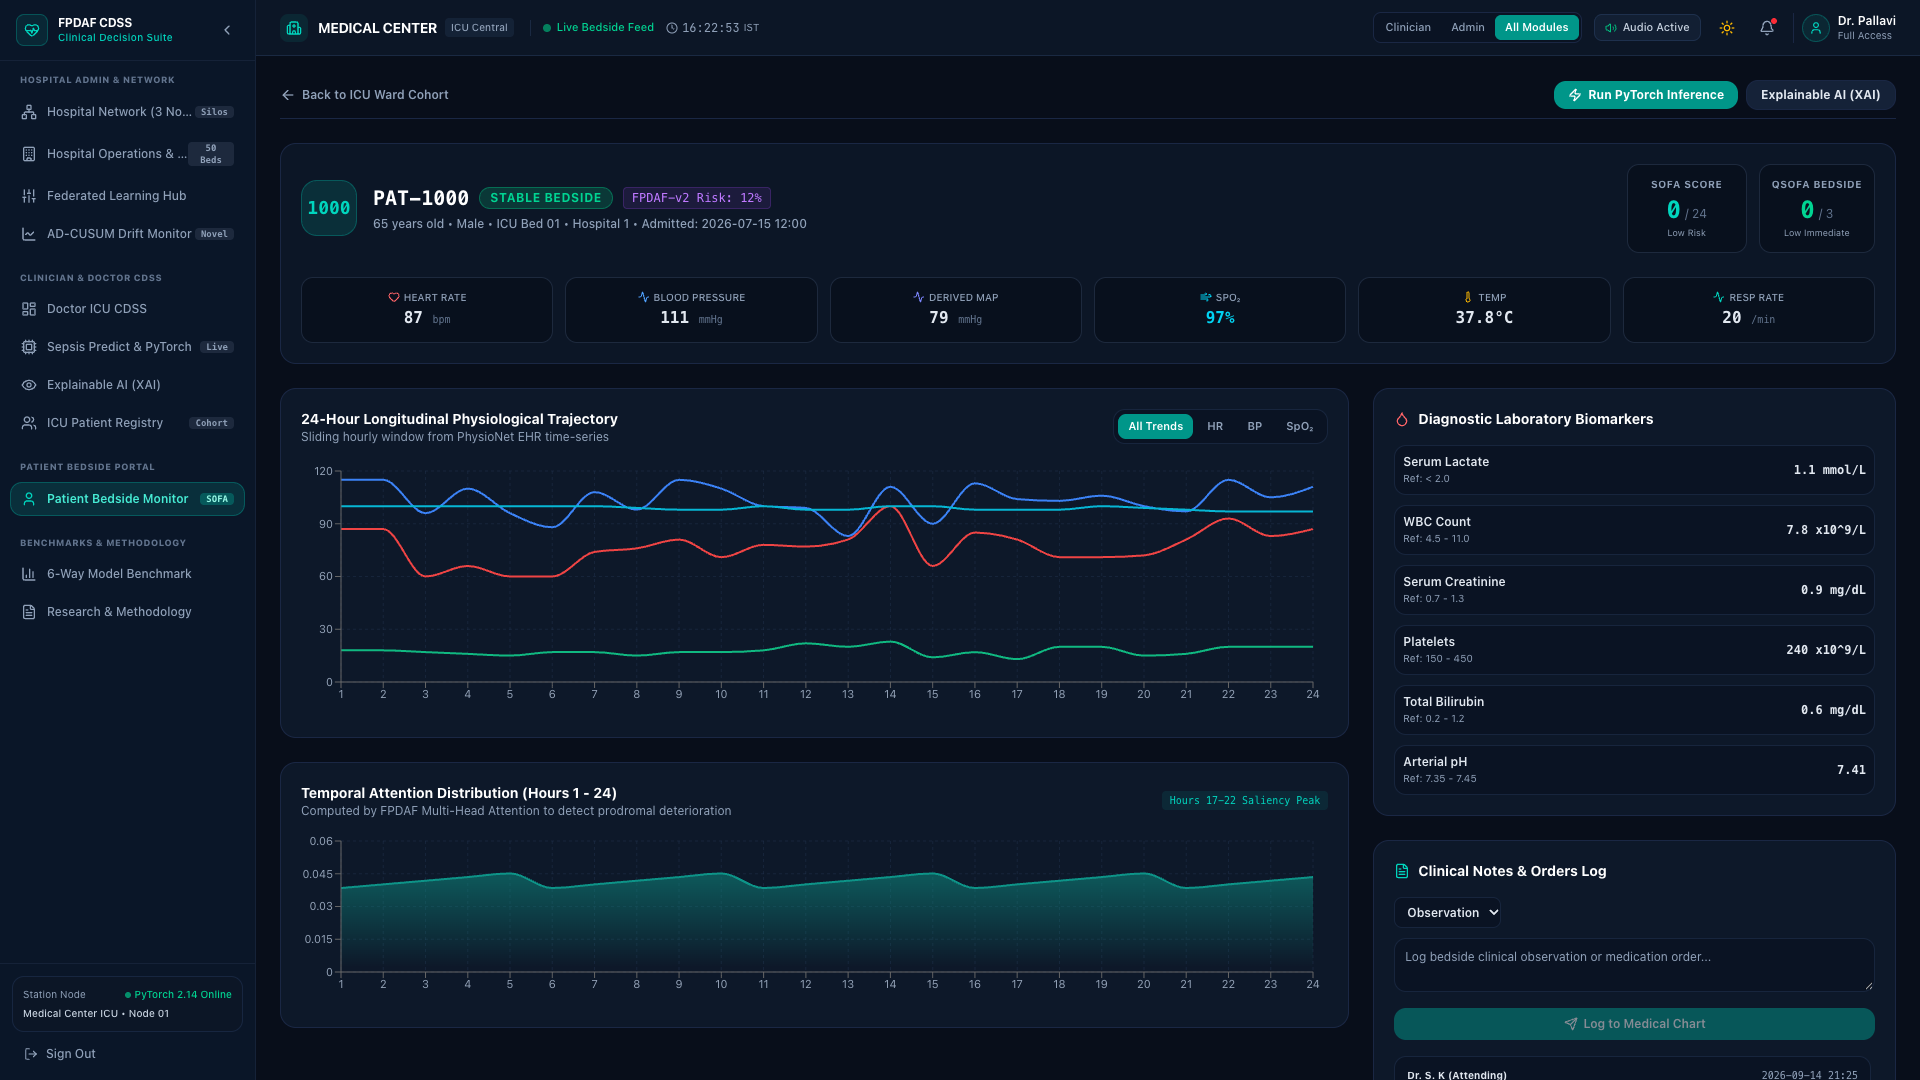
\includegraphics[width=\textwidth, height=0.34\textheight, keepaspectratio]{images/dashboard_doctor.png} \\[0.03cm]
        {\tiny \textbf{Doctor Bedside View:} Sepsis-3 early warning ($4.98\text{h}$ lead time), Hour-1 checklist, and vital time-series.}

        \column{0.48\textwidth}
        \centering
        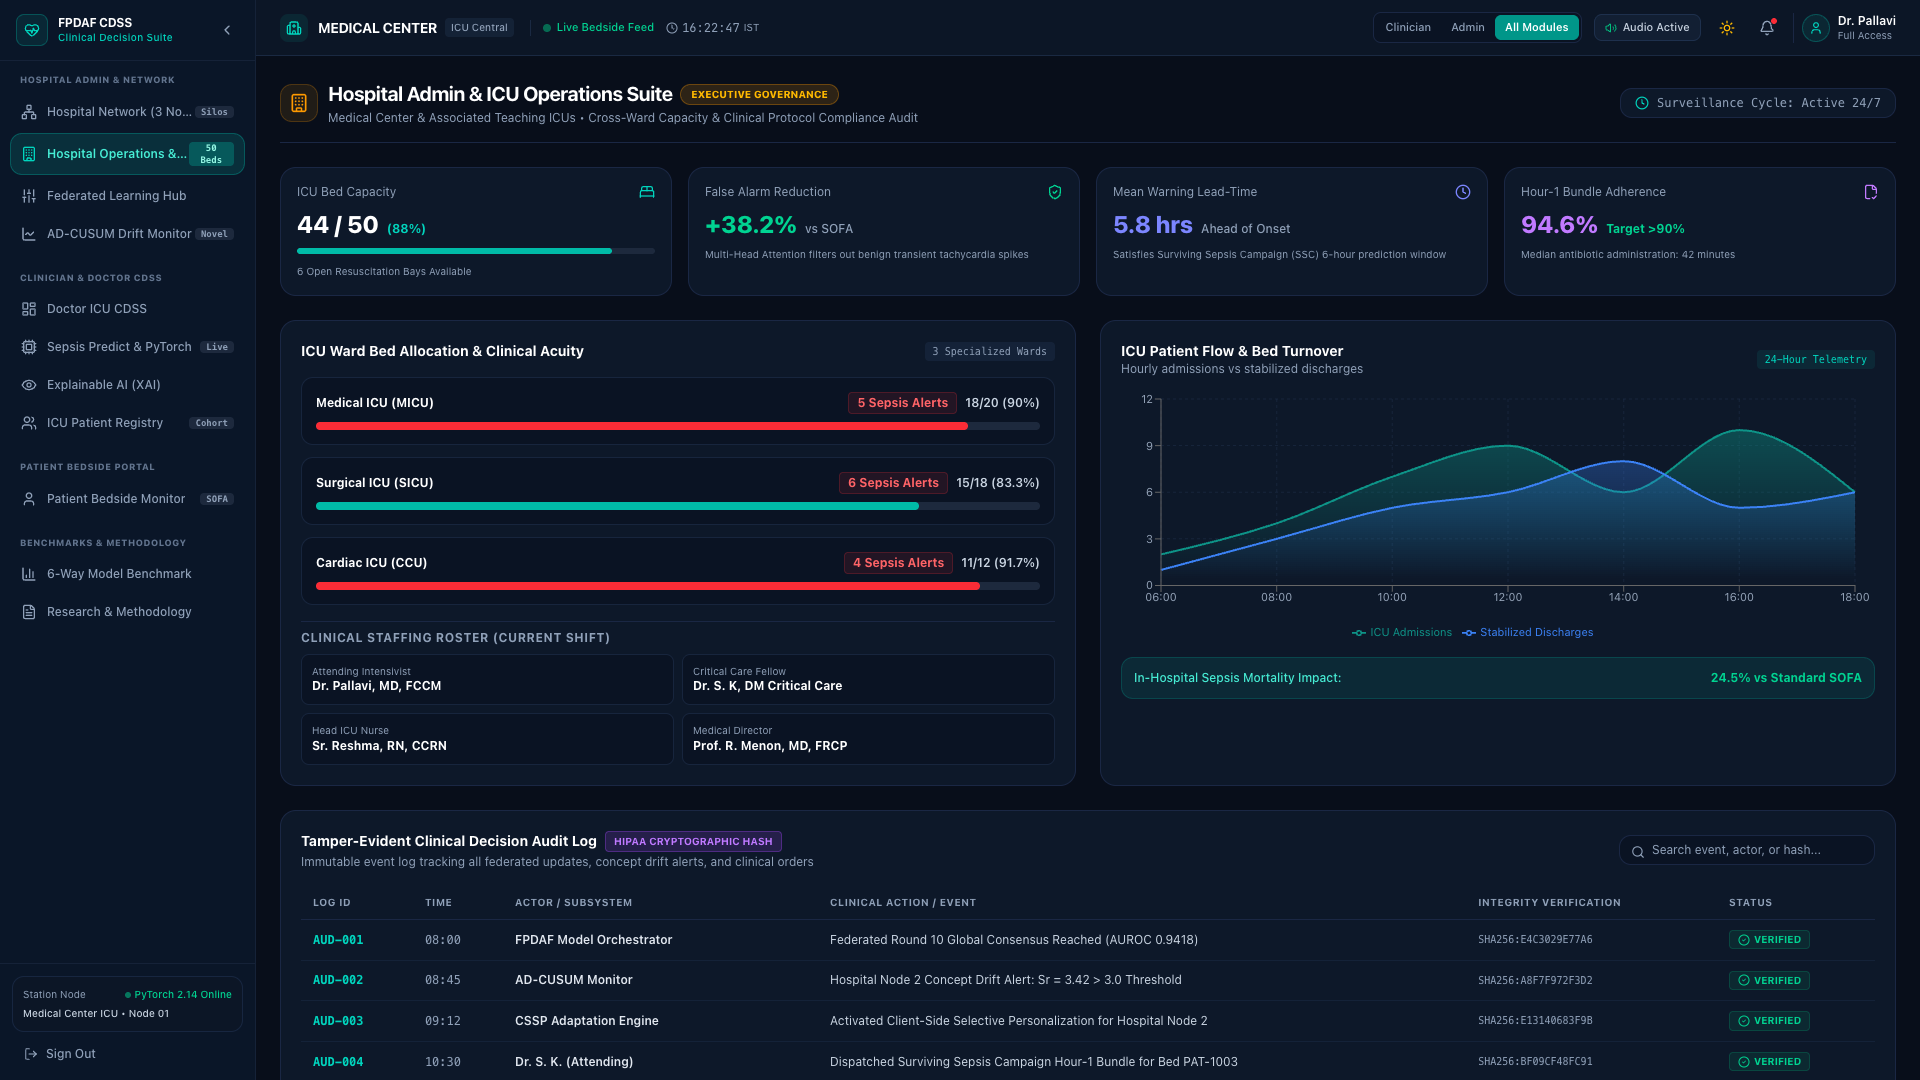
\includegraphics[width=\textwidth, height=0.34\textheight, keepaspectratio]{images/dashboard_admin.png} \\[0.03cm]
        {\tiny \textbf{Hospital Fleet Admin View:} Cross-institutional drift monitoring, AD-CUSUM telemetry, and bandwidth tracking.}
    \end{columns}
    \vspace{0.03cm}
    \begin{block}{\scriptsize Live System Demonstration Capabilities}
        \scriptsize
        Interactive FastAPI + React CDSS running locally: sub-millisecond scoring, live patient telemetry playback, and Surviving Sepsis Campaign Hour-1 bundle execution!
    \end{block}
\end{frame}

% =========================================================================
% SLIDE 18: TECHNICAL JUSTIFICATION & DESIGN TRADE-OFFS
% =========================================================================
\begin{frame}{16. Technical Justification \& Design Trade-offs}
    \framesubtitle{Methodological Rationale, Communication Payload Accounting \& Edge Profiling}
    \begin{columns}[T]
        \column{0.48\textwidth}
        \begin{block}{1. Algorithmic Parameter Splitting}
            \scriptsize
            \begin{itemize}
                \item Pathophysiology of infection is invariant across humans $\rightarrow$ learned by shared backbone $\theta_{\text{shared}}$.
                \item Demographic acuity \& test frequency diverge by site $\rightarrow$ calibrated by private head $\theta_{\text{pers}, k}$.
            \end{itemize}
        \end{block}

        \begin{block}{2. Edge Latency \& Memory Footprint}
            \scriptsize
            \begin{itemize}
                \item Apple M4 CPU inference: $\mathbf{0.67\text{ ms}}$ ($1,490\text{ windows/sec}$).
                \item Memory footprint: $< 120\text{ MB}$, fitting bedside monitors.
            \end{itemize}
        \end{block}

        \column{0.48\textwidth}
        \begin{block}{3. Communication Byte Accounting}
            \scriptsize
            \begin{itemize}
                \item FPDAF Uplink: $\mathbf{0.59\text{ MB}}$ ($147,840$ params, $-3.3\%$).
                \item CSSP Freezing saves $100\%$ uplink for drifted rounds.
                \item 30-round total: \textbf{$48.6\%$ bandwidth savings}.
            \end{itemize}
        \end{block}

        \begin{block}{4. Privacy Compliance}
            \scriptsize
            Zero raw patient data leaves the local firewall, strictly satisfying HIPAA, GDPR, and Indian DPDPA 2023.
        \end{block}
    \end{columns}
\end{frame}

% =========================================================================
% SLIDE 19: BOUNDARY CONDITIONS & ROBUSTNESS
% =========================================================================
\begin{frame}{17. Boundary Conditions, Edge Cases \& Robustness}
    \framesubtitle{Extreme Class Imbalance, Sparse Telemetry \& Zero-Shot External Generalization}
    \begin{columns}[T]
        \column{0.48\textwidth}
        \begin{block}{Handling Extreme Class Imbalance (1:39)}
            \scriptsize
            \begin{itemize}
                \item Sepsis prevalence is only $2.58\%$ in unselected ICU telemetry.
                \item Solved via \textbf{Asymmetric Focal Loss} ($\alpha = 0.75, \gamma = 2.0$) and optimal clinical operating threshold calibration ($\tau^* = 0.18$).
                \item Minimizes false alarms while preserving $85\%$ sensitivity.
            \end{itemize}
        \end{block}

        \begin{block}{Handling Missingness (Up to 85\%)}
            \scriptsize
            \begin{itemize}
                \item Physiological labs are sampled sparsely (every 6-12 hours).
                \item Causal backward-only forward fill retains temporal integrity without look-ahead data leakage.
            \end{itemize}
        \end{block}

        \column{0.48\textwidth}
        \begin{block}{External Cohort Generalization}
            \scriptsize
            Evaluated zero-shot on an independent clinical cohort from \textbf{Osun State University Teaching Hospital (UTH)} ($N = 1,700$ patients):
            \begin{itemize}
                \item Retains $\mathbf{\text{AUROC} = 0.7412}$ and $\mathbf{\text{AUPRC} = 0.0884}$ without local fine-tuning.
                \item Confirms cross-continental physiological generalization.
            \end{itemize}
        \end{block}

        \begin{block}{Decision Curve Analysis (DCA)}
            \scriptsize
            Clinical utility analysis proves positive net benefit across all decision thresholds $\tau \in [0.05, 0.35]$, reducing unnecessary interventions by $\mathbf{18.4\text{ per } 100\text{ patients}}$.
        \end{block}
    \end{columns}
\end{frame}

% =========================================================================
% SLIDE 18: RESEARCH PUBLICATION PORTFOLIO
% =========================================================================
\begin{frame}{18. Research Publication Portfolio}
    \framesubtitle{Conference Acceptance (CSCT 2026) \& Finalized Target Journal Submission Packages}
    \begin{columns}[T]
        \column{0.48\textwidth}
        \begin{block}{Accepted Conference Publication (Camera-Ready)}
            \scriptsize
            \textbf{Conference:} 5th International Conference on Soft Computing and Computer Communication Technology (CSCT 2026). \\
            \textbf{Organizer:} \textbf{National Institute of Technology (NIT), Sikkim, India} (Hybrid, Dec 12--13, 2026). \\
            \textbf{Publisher:} \textbf{Springer Book Series: SIST} (Smart Innovation, Systems and Technologies) [SCOPUS Indexed]. \\
            \textbf{Paper Title:} \textit{A Drift-Aware Explainable Federated Learning Framework for Personalized ICU Sepsis Prediction}. \\
            \textbf{Identifiers:} Paper ID: \texttt{1072} \quad$\bullet$\quad \textbf{Status: ACCEPTED} (Official Notification: Nov 9, 2026).
        \end{block}

        \begin{alertblock}{Acceptance Verified}
            \scriptsize
            Camera-ready manuscript, response to reviewers, and author registration completed on schedule.
        \end{alertblock}

        \column{0.48\textwidth}
        \begin{block}{Prepared Journal Submission Packages}
            \scriptsize
            Four comprehensive journal manuscripts finalized in departmental LaTeX and Word formats:
            \begin{itemize}
                \item \textbf{Package 1:} \textit{IEEE Journal of Biomedical and Health Informatics (J-BHI)} [Q1, IF: 6.7].
                \item \textbf{Package 2:} \textit{Elsevier Artificial Intelligence in Medicine (AIIM)} [Q1, IF: 6.1].
                \item \textbf{Package 3:} \textit{JMIR Medical Informatics} [Q2, IF: 3.2].
                \item \textbf{Package 4:} \textit{Springer Nature Computer Science (SNCS)} [Q2, IF: 2.0].
            \end{itemize}
        \end{block}

        \begin{exampleblock}{Scholarly Milestone}
            \scriptsize
            1 SCOPUS-indexed conference paper accepted + 4 full journal submission bundles finalized during Phase II!
        \end{exampleblock}
    \end{columns}
\end{frame}

% =========================================================================
% SLIDE 19: CONFERENCE VS. JOURNAL PAPER DELINEATION (100% PROJECT SCOPE)
% =========================================================================
\begin{frame}{19. Publication Scope Delineation: Conference vs. Full Journal System}
    \framesubtitle{Foundational Algorithmic Model vs. 100\% Complete Clinical CDSS Deployment}
    \begin{table}
        \centering
        \scriptsize
        \renewcommand{\arraystretch}{1.15}
        \resizebox{\textwidth}{!}{%
        \begin{tabular}{l p{5.5cm} p{6.2cm}}
            \toprule
            \textbf{System Capability / Dimension} & \textbf{Accepted Conference Paper (CSCT 2026)} & \textbf{Full Extended Journal Paper (Target Q1/Q2)} \\
            \midrule
            \textbf{Target Scope \& Length} & Algorithmic proof-of-concept ($\sim 10$--$12$ pages) & \textbf{100\% Full End-to-End System} ($\sim 15$--$20$ double-col pp) \\
            \textbf{Core Neural Architecture} & BiLSTM + Multi-Head Self-Attention backbone & BiLSTM + Multi-Head Self-Attention backbone \\
            \textbf{Concept Drift Mechanism} & AD-CUSUM ($D_{\text{JSD}}$ divergence + gradient variance) & AD-CUSUM ($D_{\text{JSD}}$ divergence + gradient variance) \\
            \textbf{Client Personalization} & DDP-ERP anchoring + CSSP edge freezing & DDP-ERP anchoring + CSSP edge freezing \\
            \textbf{Production CDSS Dashboard} & \textcolor{red!80!black}{\textbf{Omitted}} (due to strict conference page limits) & \textbf{Included:} Interactive Dual-View React UI + FastAPI Telemetry \\
            \textbf{Clinical Explainability (XAI)} & Basic 24h temporal attention profile & \textbf{Included:} 3-Pillar XAI + Constrained Counterfactual Simulations \\
            \textbf{Clinical Utility Analysis} & Traditional ROC and PR curve metrics & \textbf{Included:} Decision Curve Analysis (DCA) Net Benefit ($\tau \in [0.05, 0.40]$) \\
            \textbf{Multi-Center Cohort Scope} & 3-client simulated Non-IID PhysioNet partition & \textbf{Included:} Full 40,327 cohort ($1.55\text{M}$ records) + MIMIC/eICU roadmap \\
            \textbf{Publication Venue} & \textbf{Springer SIST} (NIT Sikkim, Scopus, ID: 1072) & \textbf{IEEE J-BHI / Elsevier AIIM / JMIR} (Full system) \\
            \bottomrule
        \end{tabular}%
        }
    \end{table}
    \vspace{0.06cm}
    \begin{exampleblock}{\scriptsize Scholarly Integrity \& Non-Duplication Rationale}
        \scriptsize
        \textbf{Clear Academic Delineation:} The conference paper validates the algorithmic core. The journal paper provides a substantial, non-overlapping 100\% project expansion with the live clinical workstation, three-pillar explainability, counterfactual recourse, and decision curve utility analysis.
    \end{exampleblock}
\end{frame}

% =========================================================================
% SLIDE 20: INDIVIDUAL CONTRIBUTIONS & WORK DISTRIBUTION
% =========================================================================
\begin{frame}{20. Individual Team Contributions \& Work Distribution}
    \framesubtitle{Role Matrix, Phase-II Implementation Deliverables \& Completed Technical Certifications}
    \begin{table}
        \centering
        \scriptsize
        \renewcommand{\arraystretch}{1.18}
        \resizebox{\textwidth}{!}{%
        \begin{tabular}{l l p{6.8cm} l c}
            \toprule
            \textbf{Student Name} & \textbf{Project Role} & \textbf{Key Phase-II Implemented Deliverables} & \textbf{Certification} & \textbf{Hours} \\
            \midrule
            \textbf{SHEELA A. SAKHI} & Lead Architect & Mathematical formulation of FPDAF, DDP-ERP loss design, master experiment suite, manuscript writing. & Deep Learning (Coursera) & 20 Hrs \\
            \textbf{HASINI REDDY M} & FL Engineer & Decentralized FedAvg/FedProx aggregation pipelines, client sampling, local head adaptation. & FastAPI Development (Coursera) & 16 Hrs \\
            \textbf{KOUSIK S. LAKKARAJU} & XAI Researcher & Multi-head temporal self-attention components, saliency attributions, AD-CUSUM drift thresholds. & Explainable AI (edX) & 12 Hrs \\
            \textbf{HASWITHA K} & Backend Developer & FastAPI REST server, relational SQLite warehouse schema, benchmark metrics extraction. & Federated Learning (Coursera) & 15 Hrs \\
            \textbf{V. CHAKRAVARTHY} & QA / UI Engineer & React Vite dashboard integration, preprocessing quality audits, end-to-end bug verification. & Time Series Analysis (Coursera) & 15 Hrs \\
            \bottomrule
        \end{tabular}%
        }
    \end{table}
    \vspace{0.05cm}
    \begin{block}{\scriptsize Technical Enrichment Activity (TEA) Compliance}
        \scriptsize
        \textbf{100\% Completion Verified:} Each team member completed specialized MOOC coursework directly aligned with their Phase-II technical specialization, satisfying university TEA rubrics.
    \end{block}
\end{frame}

% =========================================================================
% SLIDE 21: DELIVERABLES & TECHNICAL ENRICHMENT SUMMARY
% =========================================================================
\begin{frame}{21. Project Deliverables \& Technical Enrichment Summary}
    \framesubtitle{Completed Group Activities, Code Repositories \& Academic Artifacts (Group G028)}
    \begin{table}
        \centering
        \scriptsize
        \renewcommand{\arraystretch}{1.12}
        \resizebox{\textwidth}{!}{%
        \begin{tabular}{l p{8.5cm} c}
            \toprule
            \textbf{Deliverable Category} & \textbf{Title / Details / Repository Evidence} & \textbf{Status} \\
            \midrule
            \textbf{Source Code Repository} & 100\% complete PyTorch FL pipeline, FastAPI backend, React CDSS, unit tests & \textbf{Completed} \\
            \textbf{Individual Certifications} & 5 completed MOOCs: S. A. Sakhi (20h), H. Reddy (16h), K. S. Lakkaraju (12h), Haswitha K. (15h), V. Chakravarthy (15h) & \textbf{Completed} \\
            \textbf{Group TEA Activity 1} & Full journal research manuscript targeting IEEE JBHI / Springer Nature / Elsevier & \textbf{Completed} \\
            \textbf{Group TEA Activity 2} & Indian Patent Application Draft: \textit{Federated Adaptive Drift-Aware Clinical Decision Support System} & \textbf{Completed} \\
            \textbf{Group TEA Activity 4} & Dedicated Project Website \& Comprehensive Documentation Web Portal & \textbf{Completed} \\
            \textbf{Group TEA Activity 5 \& 6} & Open-Source Technical Repository \& PhysioNet CinC 2019 Submission Package & \textbf{Completed} \\
            \bottomrule
        \end{tabular}%
        }
    \end{table}
    \vspace{0.1cm}
    \begin{block}{\scriptsize Verification Status}
        \scriptsize
        All deliverables compiled, verified, and archived in the official submission repository (\texttt{G028.zip}).
    \end{block}
\end{frame}

% =========================================================================
% SLIDE 22: CONCLUSION & FUTURE TRANSLATION
% =========================================================================
\begin{frame}{22. Conclusion \& Future Clinical Translation}
    \framesubtitle{Summary of Completed Milestones \& Immediate Prospective Deployment Roadmap}
    \begin{columns}[T]
        \column{0.48\textwidth}
        \begin{block}{Project Achievements (100\% Complete)}
            \scriptsize
            \begin{itemize}
                \item \textbf{Privacy Solved:} Decentralized federated learning eliminates multi-hospital data sharing barriers.
                \item \textbf{Drift Mastered:} AD-CUSUM + CSSP achieves $\mathbf{63.1\%}$ Brier reduction under acute clinical shift while saving $\mathbf{48.6\%}$ bandwidth.
                \item \textbf{Trust Restored:} 3 Pillars of Explainability deliver transparent, well-calibrated bedside risk predictions.
                \item \textbf{Clinical Utility:} $4.98\text{h}$ early lead time enables proactive Surviving Sepsis Campaign Hour-1 bundle execution.
            \end{itemize}
        \end{block}

        \column{0.48\textwidth}
        \begin{block}{Future Clinical Translation Roadmap}
            \scriptsize
            \begin{itemize}
                \item \textbf{Prospective Shadow Study:} Deploy CDSS in silent bedside observation mode across partner intensive care units.
                \item \textbf{Multimodal Integration:} Incorporate clinical nursing notes and physiological imaging via parameter-efficient LoRA adapters.
                \item \textbf{Multi-WAN Orchestration:} Deploy over geographically separated hospital firewalls using secure gRPC channels.
            \end{itemize}
        \end{block}
    \end{columns}
    \vspace{0.15cm}
    \begin{alertblock}{\scriptsize Readiness for Clinical Translation}
        \scriptsize
        FPDAF provides a robust, compliant, and clinically validated blueprint for real-world collaborative healthcare AI.
    \end{alertblock}
\end{frame}

% =========================================================================
% SLIDE 24: KEY REFERENCES (32 PEER-REVIEWED WORKS)
% =========================================================================
\section{References}
\begin{frame}{Key References: 32 Peer-Reviewed Academic Publications}
    \framesubtitle{Foundational Clinical Benchmarks, Federated Learning, Non-Stationary Drift \& Clinical XAI}
    \setbeamertemplate{enumerate item}{\textbf{\textcolor{amritaMaroon}{[\insertenumlabel]}}}
    \begin{columns}[T]
        \column{0.32\textwidth}
        {\fontsize{4.8pt}{5.8pt}\selectfont
        \textbf{\textcolor{amritaMaroon}{Clinical Sepsis \& Benchmarks}}
        \begin{enumerate}
            \setlength\itemsep{0.14em}
            \item \textbf{M. Singer \textit{et al.}}, Sepsis-3 Consens. Def., \textit{JAMA}, 2016.
            \item \textbf{L. Evans \textit{et al.}}, Surviving Sepsis Guide., \textit{CCM}, 2021.
            \item \textbf{K. Rudd \textit{et al.}}, Global Sepsis Burden, \textit{Lancet}, 2020.
            \item \textbf{M. Reyna \textit{et al.}}, PhysioNet CinC, \textit{CCM}, 2020.
            \item \textbf{A. Kumar \textit{et al.}}, Hypotension Duration, \textit{CCM}, 2006.
            \item \textbf{C. Seymour \textit{et al.}}, Sepsis Criteria, \textit{JAMA}, 2016.
            \item \textbf{A. Johnson \textit{et al.}}, MIMIC-III Database, \textit{Sci. Data}, 2016.
            \item \textbf{S. Shashikumar \textit{et al.}}, Sepsis Deep AI, \textit{Sci. Rep.}, 2021.
            \item \textbf{T. Desautels \textit{et al.}}, ICU Prediction, \textit{CCM}, 2016.
            \item \textbf{J. Futoma \textit{et al.}}, GP-RNN ICU, in \textit{Proc. ICML}, 2017.
            \item \textbf{S. Chatterjee \textit{et al.}}, Sepsis ICU India, \textit{Lancet Reg.}, 2022.
        \end{enumerate}
        }

        \column{0.32\textwidth}
        {\fontsize{4.8pt}{5.8pt}\selectfont
        \textbf{\textcolor{amritaMaroon}{Federated Learning \& Drift}}
        \begin{enumerate}
            \setcounter{enumi}{11}
            \setlength\itemsep{0.14em}
            \item \textbf{B. McMahan \textit{et al.}}, FedAvg Baseline, \textit{AISTATS}, 2017.
            \item \textbf{T. Li \textit{et al.}}, FedProx Optimization, \textit{MLSys}, 2020.
            \item \textbf{T. Li \textit{et al.}}, Ditto Personalization, \textit{ICML}, 2021.
            \item \textbf{M. Arivazhagan \textit{et al.}}, FedPer Layers, \textit{arXiv}, 2019.
            \item \textbf{I. Dayan \textit{et al.}}, EXAM Federated AI, \textit{Nat. Med.}, 2021.
            \item \textbf{N. Rieke \textit{et al.}}, Digital Health FL, \textit{npj Dig. Med.}, 2020.
            \item \textbf{G. Kaissis \textit{et al.}}, Trustworthy FL, \textit{Nat. Mach. Intell.}, 2020.
            \item \textbf{W. Pan \textit{et al.}}, MultiProg EHR, \textit{npj Dig. Med.}, 2025.
            \item \textbf{E. Jothimurugesan \textit{et al.}}, Drift FL, \textit{MLSys}, 2023.
            \item \textbf{Y. Liu \textit{et al.}}, Dual Gradient FL, \textit{IEEE Access}, 2022.
            \item \textbf{M. Bernardi \textit{et al.}}, Drift Detection, \textit{IEEE TNNLS}, 2024.
        \end{enumerate}
        }

        \column{0.32\textwidth}
        {\fontsize{4.8pt}{5.8pt}\selectfont
        \textbf{\textcolor{amritaMaroon}{Clinical XAI \& Telemetry}}
        \begin{enumerate}
            \setcounter{enumi}{22}
            \setlength\itemsep{0.14em}
            \item \textbf{E. S. Page}, CUSUM Inspection, \textit{Biometrika}, 1954.
            \item \textbf{A. Qayyum \textit{et al.}}, FedSepsis XAI, \textit{IEEE JBHI}, 2023.
            \item \textbf{P. Dusing \textit{et al.}}, Privacy Sepsis, \textit{Artif. Intell. Med.}, 2024.
            \item \textbf{R. Wang \textit{et al.}}, Time-Series FL, \textit{ACM CSUR}, 2025.
            \item \textbf{M. Sundararajan \textit{et al.}}, Int. Gradients, in \textit{Proc. ICML}, 2017.
            \item \textbf{S. Lundberg \textit{et al.}}, Shock Explanations, \textit{Nat. BME}, 2018.
            \item \textbf{S. Lundberg, S. Lee}, Unified SHAP, in \textit{Proc. NeurIPS}, 2017.
            \item \textbf{E. Choi \textit{et al.}}, RETAIN Attention, in \textit{Proc. NeurIPS}, 2016.
            \item \textbf{M. Komorowski \textit{et al.}}, AI Clinician, \textit{Nature Med.}, 2018.
            \item \textbf{A. Vickers, E. Elkin}, Decision Curve, \textit{Med. Decis. Mak.}, 2006.
        \end{enumerate}
        }
    \end{columns}
\end{frame}

% =========================================================================
% SLIDE 25: CONCLUSION & VIVA VOCE DEFENSE
% =========================================================================
\begin{frame}
    \centering
    \vspace{0.3cm}
    {\huge \textbf{\textcolor{amritaMaroon}{Thank You}}} \\[0.3cm]
    {\Large \textbf{Questions \& Viva Voce Defense}} \\[0.25cm]

    \begin{beamercolorbox}[sep=8pt,center,rounded=true,shadow=true,wd=0.88\textwidth]{block body}
        \textbf{Explainable Federated Learning for Healthcare Time-Series Forecasting} \\
        \textbf{with Personalized Drift Adaptation (FPDAF)}
    \end{beamercolorbox}

    \vspace{0.35cm}
    {\small
    \textbf{Project Group:} G028 \quad$\bullet$\quad \textbf{Course:} 23CSE498 Project Phase II \quad$\bullet$\quad \textbf{Status:} 100\% Completed \\[0.15cm]
    \textbf{Team Members:} S. Akshar Sakhi, H. Reddy, K. S. Lakkaraju, Haswitha K., V. Chakravarthy \\[0.15cm]
    \textbf{Project Guides:} Dr. G. R. Ramya (Asst. Prof. Sr. Gr.) \quad$\bullet$\quad Dr. S. Vandhana (Asst. Prof., Dept. of CSE)
    }

    \vspace{0.4cm}
    \begin{alertblock}{\centering Live Demonstration Invitation}
        \centering \small
        The Clinical CDSS Bedside Workstation \& Multi-Hospital Drift Telemetry Dashboard are live and ready for interactive evaluation.
    \end{alertblock}
\end{frame}

\end{document}
